\documentclass{article}
\usepackage[margin=1in]{geometry}
\usepackage[utf8]{inputenc}
\usepackage{amsfonts,amsmath,bm}
\usepackage{xcolor}
\usepackage{graphicx}
\usepackage{caption}
\usepackage{subcaption}
\usepackage{tabulary}
\usepackage{multirow}
\usepackage{algorithm}
\usepackage{algpseudocode}
\usepackage{hyperref}
% color def
\usepackage{color}
\definecolor{darkred}{rgb}{0.6,0.0,0.0}
\definecolor{darkgreen}{rgb}{0,0.50,0}
\definecolor{lightblue}{rgb}{0.0,0.42,0.91}
\definecolor{orange}{rgb}{0.99,0.48,0.13}
\definecolor{grass}{rgb}{0.18,0.80,0.18}
\definecolor{pink}{rgb}{0.97,0.15,0.45}

% listings
\usepackage{listings}

% General Setting of listings
\lstset{
  aboveskip=1em,
  breaklines=true,
  abovecaptionskip=-6pt,
  captionpos=b,
  escapeinside={\%*}{*)},
  frame=single,
  numbers=left,
  numbersep=15pt,
  numberstyle=\tiny,
}
% 0. Basic Color Theme
\lstdefinestyle{colored}{ %
  basicstyle=\ttfamily,
  backgroundcolor=\color{white},
  commentstyle=\color{green}\itshape,
  keywordstyle=\color{blue}\bfseries\itshape,
  stringstyle=\color{red},
}
% 1. General Python Keywords List
\lstdefinelanguage{PythonPlus}[]{Python}{
  morekeywords=[1]{,as,assert,nonlocal,with,yield,self,True,False,None,} % Python builtin
  morekeywords=[2]{,__init__,__add__,__mul__,__div__,__sub__,__call__,__getitem__,__setitem__,__eq__,__ne__,__nonzero__,__rmul__,__radd__,__repr__,__str__,__get__,__truediv__,__pow__,__name__,__future__,__all__,}, % magic methods
  morekeywords=[3]{,object,type,isinstance,copy,deepcopy,zip,enumerate,reversed,list,set,len,dict,tuple,range,xrange,append,execfile,real,imag,reduce,str,repr,}, % common functions
  morekeywords=[4]{,Exception,NameError,IndexError,SyntaxError,TypeError,ValueError,OverflowError,ZeroDivisionError,}, % errors
  morekeywords=[5]{,ode,fsolve,sqrt,exp,sin,cos,arctan,arctan2,arccos,pi, array,norm,solve,dot,arange,isscalar,max,sum,flatten,shape,reshape,find,any,all,abs,plot,linspace,legend,quad,polyval,polyfit,hstack,concatenate,vstack,column_stack,empty,zeros,ones,rand,vander,grid,pcolor,eig,eigs,eigvals,svd,qr,tan,det,logspace,roll,min,mean,cumsum,cumprod,diff,vectorize,lstsq,cla,eye,xlabel,ylabel,squeeze,}, % numpy / math
}
% 2. New Language based on Python
\lstdefinelanguage{PyBrIM}[]{PythonPlus}{
  emph={d,E,a,Fc28,Fy,Fu,D,des,supplier,Material,Rectangle,PyElmt},
}
% 3. Extended theme
\lstdefinestyle{colorEX}{
  basicstyle=\ttfamily,
  backgroundcolor=\color{white},
  commentstyle=\color{darkgreen}\slshape,
  keywordstyle=\color{blue}\bfseries\itshape,
  keywordstyle=[2]\color{blue}\bfseries,
  keywordstyle=[3]\color{grass},
  keywordstyle=[4]\color{red},
  keywordstyle=[5]\color{orange},
  stringstyle=\color{darkred},
  emphstyle=\color{pink}\underbar,
}
% \usepackage{biblatex}
% \addbibresource{bibliography.bib} %Import the bibliography file
% \usepackage[framed,numbered,autolinebreaks,useliterate]{mcode}
\usepackage{tikz}
\newcommand*\circled[1]{\tikz[baseline= (char.base)]{
            \node[shape=circle, draw, inner sep=1.5pt] (char) {#1};}}
\newcommand*\smallcircled[1]{\tikz[baseline= (char.base)]{
            \node[shape=circle, draw, inner sep=0.5pt] (char) {#1};}}


\title{EEC269A - Error Correcting Codes I\\Project Report}
\author{Chenye Yang, Pranav Kharche, Parisa Oftadeh}
\date{\today}

\begin{document}

\maketitle

\tableofcontents














\newpage
\section{Workload}

\begin{table}[htb]
    \centering
    \caption{Workload}
    \label{tab:workload}
    \renewcommand{\arraystretch}{1.5}
    \begin{tabulary}{\textwidth}{ |L|L|L| } 
    \hline
    \textbf{Function} & \textbf{Workload} & \textbf{Contributor} \\
    \hline
    Src \& Dest & Text string (TXT), Image (PNG), Audio (WAV) & Chenye \\ 
    \hline
    \multirow{2}{*}{Encoder \& Decoder} & $(7,4)$ Systematic Linear Block (Hamming) Code & \multirow{2}{*}{Chenye} \\ 
    & $(n,k)$ Systematic Cyclic Code & \\ 
    \hline
    Channel & Binary Symmetric Channel (BSC), adjustable error prob $p$ & Chenye \\ 
    \hline
    \multirow{3}{*}{Error Corrector} &  Syndrome Lookup Table for $(7,4)$ Linear Code & Chenye \\ 
    & Syndrome Lookup Table for $(n,k)$ Cyclic Code, $t=1$ & Chenye \\ 
    & Error Trapping for $(n,k)$ Cyclic Code, adjustable $t$ & Pranav \\
    \hline
    \multirow{2}{*}{\textbf{Advanced features}} & \textbf{Create generator matrix for $(n,k)$ cyclic code} & \multirow{2}{*}{Pranav} \\ 
    & \textbf{Adjustable: $(n,k)$ and correctable errors $t$} &  \\
    \hline
    \textbf{Data Analysis} & \textbf{Statistic Results} & Parisa, Chenye \\ 
    \hline
    \textbf{Presentation} & Slides & Parisa \\ 
    \hline
    \textbf{Report} & Work together & - \\
    \hline
    \end{tabulary}
\end{table}



\section{Source \& Destination}
\subsection{Source}

\subsubsection{Text string}
The very basic function of the information source is to read a hard-coded text file into a bit stream. 
In our text file, the following string is stored in ASCII format:
\begin{center}
    Hello World!\\EEC269A Error Correcting Code Demo
\end{center}
In ASCII format, each character is represented by 8 bits, shown in Table~\ref{tab:ascii}. Then, after transformation, the bit stream is of size 376 bits: 
\begin{center}
    0 1 0 0 1 0 0 0 0 1 1 0 0 1 0 1 \dots
\end{center}

\begin{table}[ht]
    \centering
    \caption{ASCII Table example}
    \label{tab:ascii}
    \begin{tabulary}{\textwidth}{|L|L|L|L|}
    \hline
    Character & Hexadecimal & Decimal & Binary \\
    \hline
    \dots & \dots & \dots & \dots \\
    \hline
    A & 41 & 65 & 0 1 0 0 0 0 0 1 \\
    \hline
    B & 42 & 66 & 0 1 0 0 0 0 1 0 \\
    \hline
    C & 43 & 67 & 0 1 0 0 0 0 1 1 \\
    \hline
    D & 44 & 68 & 0 1 0 0 0 1 0 0 \\
    \hline
    E & 45 & 69 & 0 1 0 0 0 1 0 1 \\
    \hline
    F & 46 & 70 & 0 1 0 0 0 1 1 0 \\
    \hline
    G & 47 & 71 & 0 1 0 0 0 1 1 1 \\
    \hline
    H & 48 & 72 & 0 1 0 0 1 0 0 0 \\
    \hline
    \dots & \dots & \dots & \dots \\
    \hline
    \end{tabulary}
\end{table}


\subsubsection{Image}
PNG (Portable Network Graphics) is a raster graphics file format that supports lossless data compression. 
PNG supports a large number of colors (up to 16 million), as well as variable transparency, which makes it useful for images with varying degrees of transparency or opacity. 
Additionally, because PNG is a lossless format, it preserves all the detail in the original image, which is not the case with lossy formats like JPEG. 
It is used for the storage and display of images on the internet, and is also used in graphic design and editing applications due to its lossless compression.

PNG files consist of a header followed by a series of data chunks, e.g.:
\begin{enumerate}
    \item Signature: The first eight bytes of a PNG file always contain the following decimal numbers: 137, 80, 78, 71, 13, 10, 26, 10. This signature indicates that the file is a PNG.
    \item Header Chunk (IHDR): The first chunk after the signature is the IHDR chunk, which contains basic information about the image, such as width, height, bit depth, color type, compression method, filter method, and interlace method.
    \item Palette Chunk (PLTE): This chunk is optional and only present for color type 3 (indexed color). It contains the color palette for the image.
    \item Data Chunks (IDAT): These chunks contain the actual image data, which is formed by pixels. This data is compressed to reduce the size of the file.
    \item End Chunk (IEND): This is the final chunk in a PNG file. It does not contain any data and its purpose is to indicate the end of the file.
\end{enumerate}
Each chunk contains three standard fields: 4-byte length, 4-byte type code, 4-byte CRC and various internal fields that depend on the chunk type, shown in Figure~\ref{fig:png-structure} \footnote{Figure~\ref{fig:png-structure} is from webpage \href{https://www.nayuki.io/res/dumb-png-output-java/png-file-format.svg}{PNG file chunk inspector - Project Nayuki}}. 
For example, the image file we are using has more than one image data (IDAT) chunks, each of which contains a portion of the image, shown in Table~\ref{tab:our-png-structure}.

\begin{figure}[htb]
    \centering
    \hfill
    \begin{minipage}[b]{0.3\textwidth}
        \includegraphics[width=\textwidth]{png-file-format.png}
        \caption{PNG file structure}
    \label{fig:png-structure}
    \end{minipage}
    \hfill
    \begin{minipage}[b]{0.36\textwidth}
        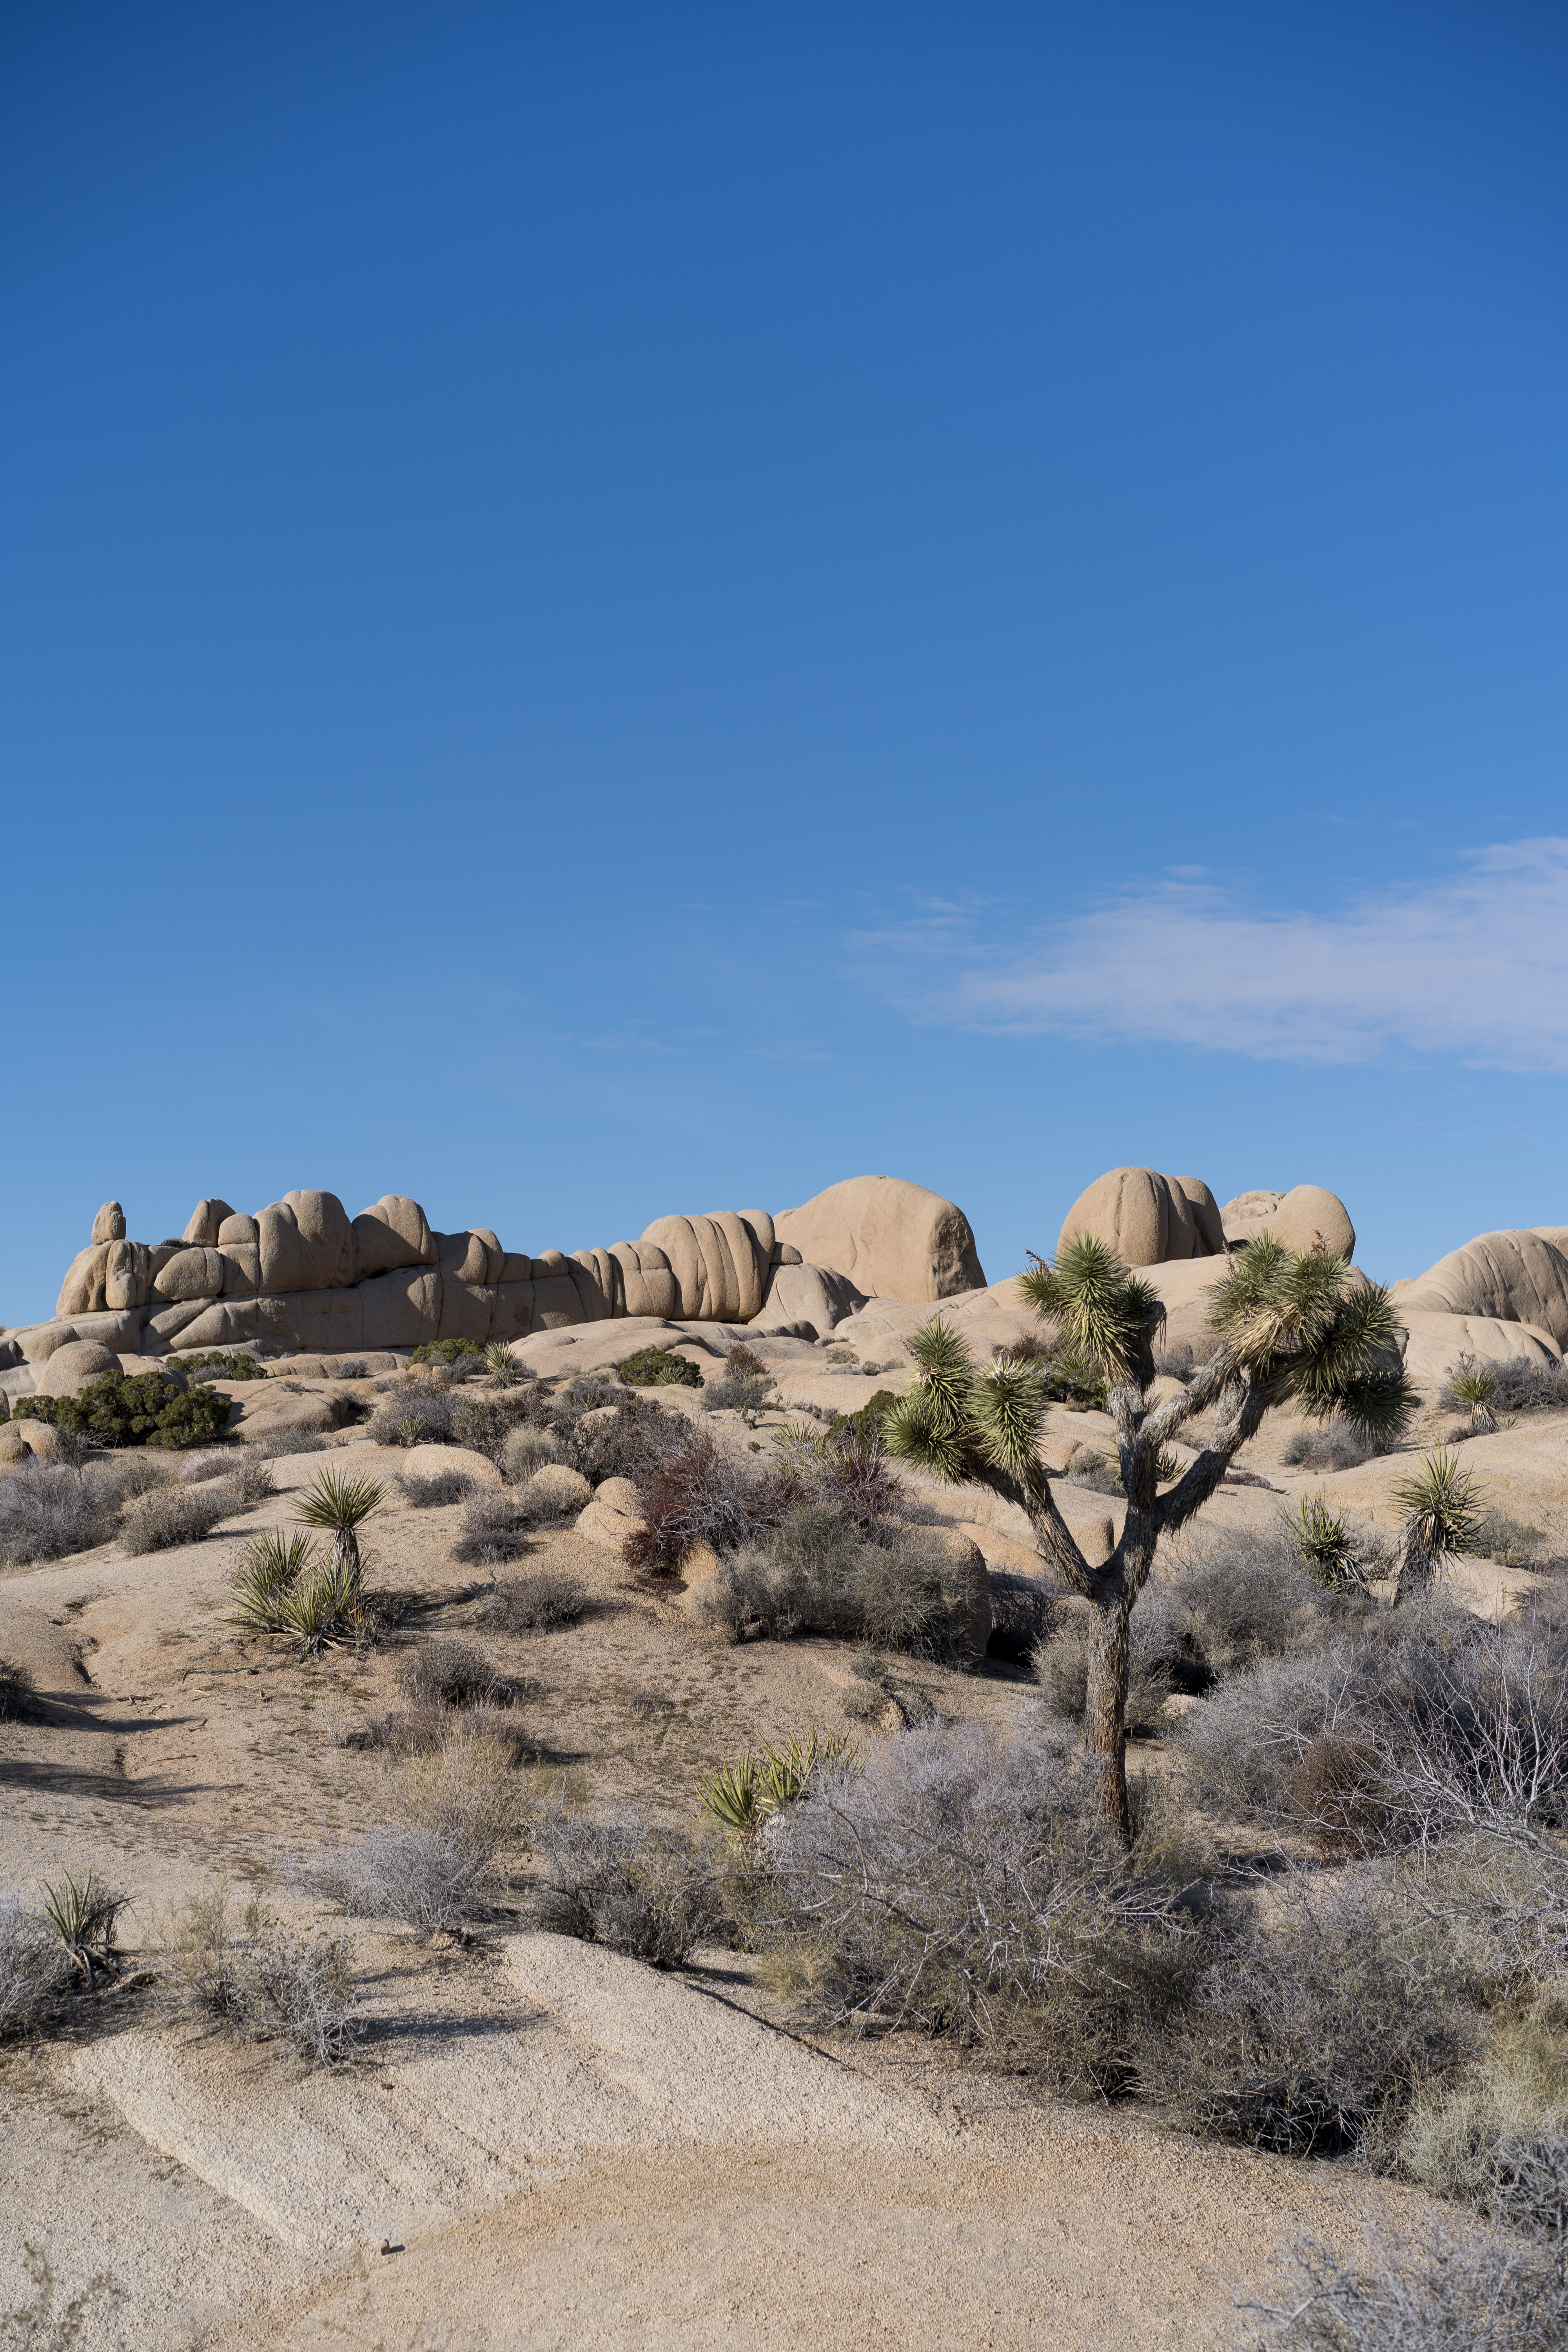
\includegraphics[width=\textwidth]{../Resource/image.png}
        \caption{Our testing PNG image}
    \label{fig:our-image}
    \end{minipage}
    \hfill
\end{figure}


\begin{table}[htb]
    \centering
    \caption{Our PNG file structure}
    \label{tab:our-png-structure}
    \renewcommand{\arraystretch}{1.5}
    \begin{tabulary}{\textwidth}{ |L|L| } 
    \hline
    Start offset & Chunk outside \\
    \hline
    0 & Special: File signature; Length: 8 bytes \\
    \hline
    8 & Data length: 13 bytes; Type: IHDR; Name: Image header; CRC-32: CB3954EC \\
    \hline
    33 & Data length: 1 bytes; Type: sRGB; Name: Standard RGB color space; CRC-32: AECE1CE9 \\
    \hline
    46 & Data length: 976 bytes; Type: eXIf; Name: Exchangeable Image File (Exif) Profile; CRC-32: 47FCFA4D \\
    \hline
    1,034 & Data length: 9 bytes; Type: pHYs; Name: Physical pixel dimensions; CRC-32: 5024E7F8 \\
    \hline
    1,055 & Data length: 4 514 bytes; Type: iTXt; Name: International textual data; CRC-32: C9C76B16 \\
    \hline
    5,581 & Data length: 16 384 bytes; Type: IDAT; Name: Image data; CRC-32: 8462CABD \\
    \hline
    21,977 & Data length: 16 384 bytes; Type: IDAT; Name: Image data; CRC-32: 2C9D007C \\
    \hline
    \dots & \dots \\
    \hline
    1,727,161 & Data length: 12 170 bytes; Type: IDAT; Name: Image data; CRC-32: 68067F52 \\
    \hline
    1,739,343 & Data length: 0 bytes; Type: IEND; Name: Image trailer; CRC-32: AE426082 \\
    \hline
    \end{tabulary}
\end{table}

Ideally, the entire image file should be read into a bit stream and transmitted through the channel. 
However, if there are uncorrectable errors in the chunks other than the image data (IDAT), the received image will not be able to display.
Therefore, we shall only work with the image data (IDAT) chunks for the purpose of visualization of a corrupted image. 
Also, this trick will not affect the statistical analysis of the system. 

The information source is able to only extract the color information from a PNG file and convert it into a bit stream to be passed through the channel. 
This is done by using the Python library \textit{NumPy}.

The library \textit{NumPy} provides a method to only read out the color information of an image. The shape of the result array is typically \textit{(height, width, channels)}, where:
\begin{enumerate}
    \item \textit{height} is the number of pixels in the vertical direction (i.e. the number of rows of pixels);
    \item \textit{width} is the number of pixels in the horizontal direction (i.e. the number of columns of pixels);
    \item \textit{channels} is the number of color channels per pixel. This value depends on what type of image it is: \begin{itemize}
        \item In an RGB image, the three channels correspond to Red, Green, and Blue, respectively. Each channel value usually ranges from 0 to 255, where 0 indicates none of that color is present and 255 indicates that color is fully present.
        \item In a grayscale image, there is typically only one channel. The value in this single channel indicates the level of gray, where 0 is black and 255 is white.
        \item There are many other color spaces that have different meanings for their channels.
    \end{itemize}
\end{enumerate}
The data type for each channel of each pixel is \textit{uint8}, which is an unsigned integer that takes 8 bits.
Then, the array is flattened into a bit stream by converting each channel of each pixel into an 8-bits binary number and appending them together.

For example, as for our testing image\footnote{The image file used in this project is photographed by \textit{Chenye Yang}. The material is free from any copyright restrictions and can be used without any potential legal implications.}, shown in Figure~\ref{fig:our-image}, the shape of the result array is \textit{(1280, 854, 3)}, which means that the image has 1280 rows of pixels, 854 columns of pixels, and 3 color channels per pixel (RGB). 
Then, the array is flattened into a bit stream of 26,234,880 bits.







\subsubsection{Audio}
WAV (Waveform Audio File Format) is a digital audio standard for storing audio bitstream on PCs. 
WAV is an application of the Resource Interchange File Format (RIFF) method for storing data in chunks, and it is primarily used on Windows systems. 
WAV files are typically used for raw and uncompressed audio, though they can also contain compressed audio.
A WAV file is divided into several sections or chunks, shown in Figure~\ref{fig:canonical-wav-structure} \footnote{Figure~\ref{fig:canonical-wav-structure} is from webpage \href{https://www.videoproc.com/resource/wav-file.htm}{WAV Files: File Structure, Case Analysis and PCM Explained}}. Each chunk serves a different purpose and holds different types of data. The basic structure of a WAV file includes the following chunks:
\begin{enumerate}
    \item RIFF Chunk: The RIFF chunk is the first chunk in a WAV file and identifies the file as a WAV file. It includes a header with the "RIFF" identifier and an integer indicating the remaining length of the entire file.
    \item Format Chunk: Also known as the "fmt " chunk (with a space after 'fmt'), this contains important information about the audio data. This includes the audio format (e.g., PCM), the number of channels (mono, stereo, etc.), the sample rate, the byte rate, the block alignment, and the bit depth (bits per sample).
    \item Data Chunk: This is where the actual audio data is stored. The "data" header is followed by an integer representing the length of the data, and then by the raw audio data itself.
\end{enumerate}


\begin{figure}[htb]
    \centering
    \includegraphics[width=0.7\textwidth]{canonical-wav-file-structure.jpg}
    \caption{Canonical WAV file structure}
    \label{fig:canonical-wav-structure}
\end{figure}

Similar to the image file, the information source is able to only extract the audio Data Chunk from a WAV file and convert it into a bit stream to be passed through the channel. 
This trick ensures both the visualization of the results and the statistical analysis of the system. The extraction is done by using the Python library \textit{soundfile}.

The library \textit{soundfile} provides a method to only read out the audio data from a WAV file. The result contains two parts:
\begin{enumerate}
    \item audio array: This is a \textit{NumPy} array that contains the audio data from the file. The shape of the array depends on the number of channels in the audio file. If the audio is mono, the array will be one-dimensional. If the audio is stereo, the array will be two-dimensional, with one sub-array for each channel. The values in the array represent the amplitude of the audio signal at each sample point, and are of the data type specified.
    \item sample rate: This is an integer that represents the number of samples per second in the audio file, measured in Hertz (Hz). Common sample rates include 44100 Hz (standard for audio CDs), 48000 Hz (standard for video production and DVDs), and 96000 Hz (used in high-definition formats).
\end{enumerate}
Then, the \textit{int16} array is "viewed" as \textit{uint8} array by \textit{numpy.view()} and flattened into a bit stream by converting each sample into an 8-bits binary number and appending them together. 
Note that the \textit{numpy.view()} operation simply reinterprets the binary data, and does not convert or scale the data, which originally could be negative or positive. 

For example, as for our testing audio file\footnote{The audio file used in this project is free downloaded from \href{https://file-examples.com/index.php/sample-audio-files/sample-wav-download/}{file-examples.com}. The material is free from any copyright restrictions and can be used without any potential legal implications.}, shown in Figure~\ref{fig:our-audio-time-domain} and Figure~\ref{fig:our-audio-frequency-domain}, 
the shape of the result audio array is \textit{(268237, 2)} and the sample rate is 8000 Hz. It means that the 33.5-second audio file has 268237 samples per channel, and there are two channels (stereo). 
Then, the array is flattened into a bit stream of 8,583,584 bits.


\begin{figure}[htb]
    \centering
    \includegraphics[width=\textwidth]{../Result/Linear/wav-time-domain-TX.png}
    \caption{Time domain waveform of our testing audio file}
    \label{fig:our-audio-time-domain}
\end{figure}

\begin{figure}[htb]
    \centering
    \includegraphics[width=\textwidth]{../Result/Linear/wav-frequency-domain-TX.png}
    \caption{Frequency domain waveform of our testing audio file}
    \label{fig:our-audio-frequency-domain}
\end{figure}







\subsection{Destination}
At the destination, the bit stream is re-construed into the original format, and stored. 
It is inevitable that some metadata is lost when processed by the system, since they are not transmitted through the channel.
For example, the re-constructed image file will not have the camera and lens information. 
However, this is the trade-off for a better visualization, and will not affect the statistical analysis of the system.








\section{Channel}

\subsection{Binary Symmetric Channel (BSC)}
The Binary Symmetric Channel (BSC) is a fundamental concept in information theory and telecommunications, specifically in the field of error detection and correction. It is a model used to represent a communication channel, where the information is transmitted in the form of binary digits, or bits: 0s and 1s.

The "symmetric" aspect of the BSC refers to the fact that it has the same probability of an error occurring whether the transmitted bit is a 0 or a 1. For instance, if the error probability is 0.01, then 1\% of 0s are received as 1s, and 1\% of 1s are received as 0s. 

A BSC is characterized by two parameters: the input bit and the crossover probability / error probability, shown in Figure~\ref{fig:bsc}. The input bit is either 0 or 1, which represents the binary information being transmitted. The crossover probability, often denoted as $p$, represents the likelihood of the transmitted bit being received incorrectly. 

Although the model is simple, the BSC is a building block for understanding more complex communication systems. By studying the BSC, researchers can develop algorithms and systems that minimize errors in binary data transmission, improving the reliability of digital communications.

All the results are done with error probability $p = 0.01$, even though this $p$ is a configurable value in $[0, 1]$ by users.

\begin{figure}[htb]
    \centering
    \includegraphics[width=0.3\textwidth]{bsc.png}
    \caption{Binary Symmetric Channel (BSC)}
    \label{fig:bsc}
\end{figure}
















\section{(7,4) Systematic Linear Block (Hamming) Code}
The (7,4) Systematic Linear Block (Hamming) Code, often referred to simply as the Hamming (7,4) Code, is a fundamental concept in the realm of error detection and correction, and plays a crucial role in the field of digital communications and information theory. This coding scheme was introduced by Richard Hamming in the late 1940s to address the problem of error detection and correction in data transmission over noisy channels.

The Hamming (7,4) Code is a block code that maps 4-bit messages to 7-bit codewords. It gets its name from the fact that it takes in 4 data bits and outputs 7 bits (including 3 parity bits). The parity bits are extra bits added to the data to enable the detection and correction of errors that might occur during transmission.

A key characteristic of the Hamming (7,4) Code is its systematic form. This means that the bits of the original message appear unaltered in the encoded output, making it easy to extract the original data from the received message, even if errors are detected. 

The Hamming (7,4) Code is designed to detect and correct single-bit errors, meaning it can identify and fix any situation where only one bit in the 7-bit codeword has been flipped due to noise or interference in the communication channel. This makes it a powerful tool in improving the reliability and robustness of data communication systems.



\subsection{Encoder}
The encoding process in a Hamming (7,4) code involves the multiplication of a 4-bit message vector with a generator matrix. The generator matrix for a (7,4) Hamming Code, in its systematic form, is given as:
\begin{equation*}
    G = 
        \begin{bmatrix}
        1 & 1 & 0 & 1 & 0 & 0 & 0 \\
        0 & 1 & 1 & 0 & 1 & 0 & 0 \\
        1 & 1 & 1 & 0 & 0 & 1 & 0 \\
        1 & 0 & 1 & 0 & 0 & 0 & 1 \\
        \end{bmatrix}.
\end{equation*}

If we denote the message vector as 
\begin{equation*}
    u =
        \begin{bmatrix}
        u_1 & u_2 & u_3 & u_4 
        \end{bmatrix},
\end{equation*}
then the encoded codeword $v$ is computed by:
\begin{equation*}
    v = u \cdot G .
\end{equation*}

This multiplication produces a 7-bit codeword, which is then ready for transmission.





\subsection{Syndrome Decoder}
First, the parity-check matrix $H$ will be created from the generator matrix $G$ by transposing the 4 by 3 parity-check bits and filling it with an 3 by 3 identity matrix:
\begin{equation*}
H = 
\begin{bmatrix}
1 & 0 & 0 & 1 & 0 & 1 & 1 \\
0 & 1 & 0 & 1 & 1 & 1 & 0 \\
0 & 0 & 1 & 0 & 1 & 1 & 1 \\
\end{bmatrix} .
\end{equation*}

The decoding process of the (7,4) Hamming code involves utilizing a syndrome lookup table, which is generated from the matrix multiplication:
\begin{equation*}
\text{syndrome table} = e \cdot H^T = \begin{bmatrix}
0 & 0 & 0 & 0 & 0 & 0 & 0 \\
1 & 0 & 0 & 0 & 0 & 0 & 0 \\
0 & 1 & 0 & 0 & 0 & 0 & 0 \\
0 & 0 & 1 & 0 & 0 & 0 & 0 \\
0 & 0 & 0 & 1 & 0 & 0 & 0 \\
0 & 0 & 0 & 0 & 1 & 0 & 0 \\
0 & 0 & 0 & 0 & 0 & 1 & 0 \\
0 & 0 & 0 & 0 & 0 & 0 & 1 \\
\end{bmatrix} \cdot H^T
= \begin{bmatrix}
    0 & 0 & 0 \\
    1 & 0 & 0 \\
    0 & 1 & 0 \\
    0 & 0 & 1 \\
    1 & 1 & 0 \\
    0 & 1 & 1 \\
    1 & 1 & 1 \\
    1 & 0 & 1 \\
\end{bmatrix} ,
\end{equation*}
where the 7 by 7 identity matrix with an extra row of zeros on the top, $e$, represents all the possible error patterns which are correctable by a syndrome look-up table for this specific (7,4) hamming code with generator matrix $G$. Each row of $e$ represents an error pattern identified by the same row of syndrome table. 

When a codeword is received, the syndrome $s$ is computed from the received bits and is used to identify the error pattern:
\begin{equation*}
    s = r \cdot H^T ,
\end{equation*}
where the $r = [r_1\  r_2\  \dots\  r_7 ]$ represents the received codeword. 

Each syndrome corresponds to a potential error pattern in the look-up table. The estimated transmitted codeword can be calculated by modulo 2 addiction of error pattern and received codeword:
\begin{equation*}
    \tilde{v} = r + e[i:] \mod 2 ,
\end{equation*}
where the $e[i:]$ represents the $i$-th row of error patterns $e$ when the calculated syndrome $s$ matches the $i$-th row of the syndrome table. 

Since the code we are working on is systematic code, messages can be directly extracted from the last 4 bits of codewords. 


\subsubsection{Results: TXT, PNG, WAV}
Shown in Table~\ref{tab:text-linear} Figure~\ref{fig:image-linear}~
\begin{table}[htb]
    \centering
    \caption{Text string encoded with (7, 4) linear Hamming code}
    \label{tab:text-linear}
    \renewcommand{\arraystretch}{1.5}
    \begin{tabulary}{\textwidth}{ |L|L|L| } 
    \hline
    \textbf{Original} & \textbf{Without correction} & \textbf{Corrected} \\
    \hline
    Hello World! EEC269A Error Correcting Code Demo & Hello Wo\textcolor{red}{p}ld! EEC269A \textcolor{red}{A}rror Correcting \textcolor{red}{K}ode Demo & Hello World! EEC269A Error Correcting Code Demo \\
    \hline
    \end{tabulary}
\end{table}


\begin{figure}[htb]
    \centering
    \begin{subfigure}[b]{0.32\textwidth}
        \centering
        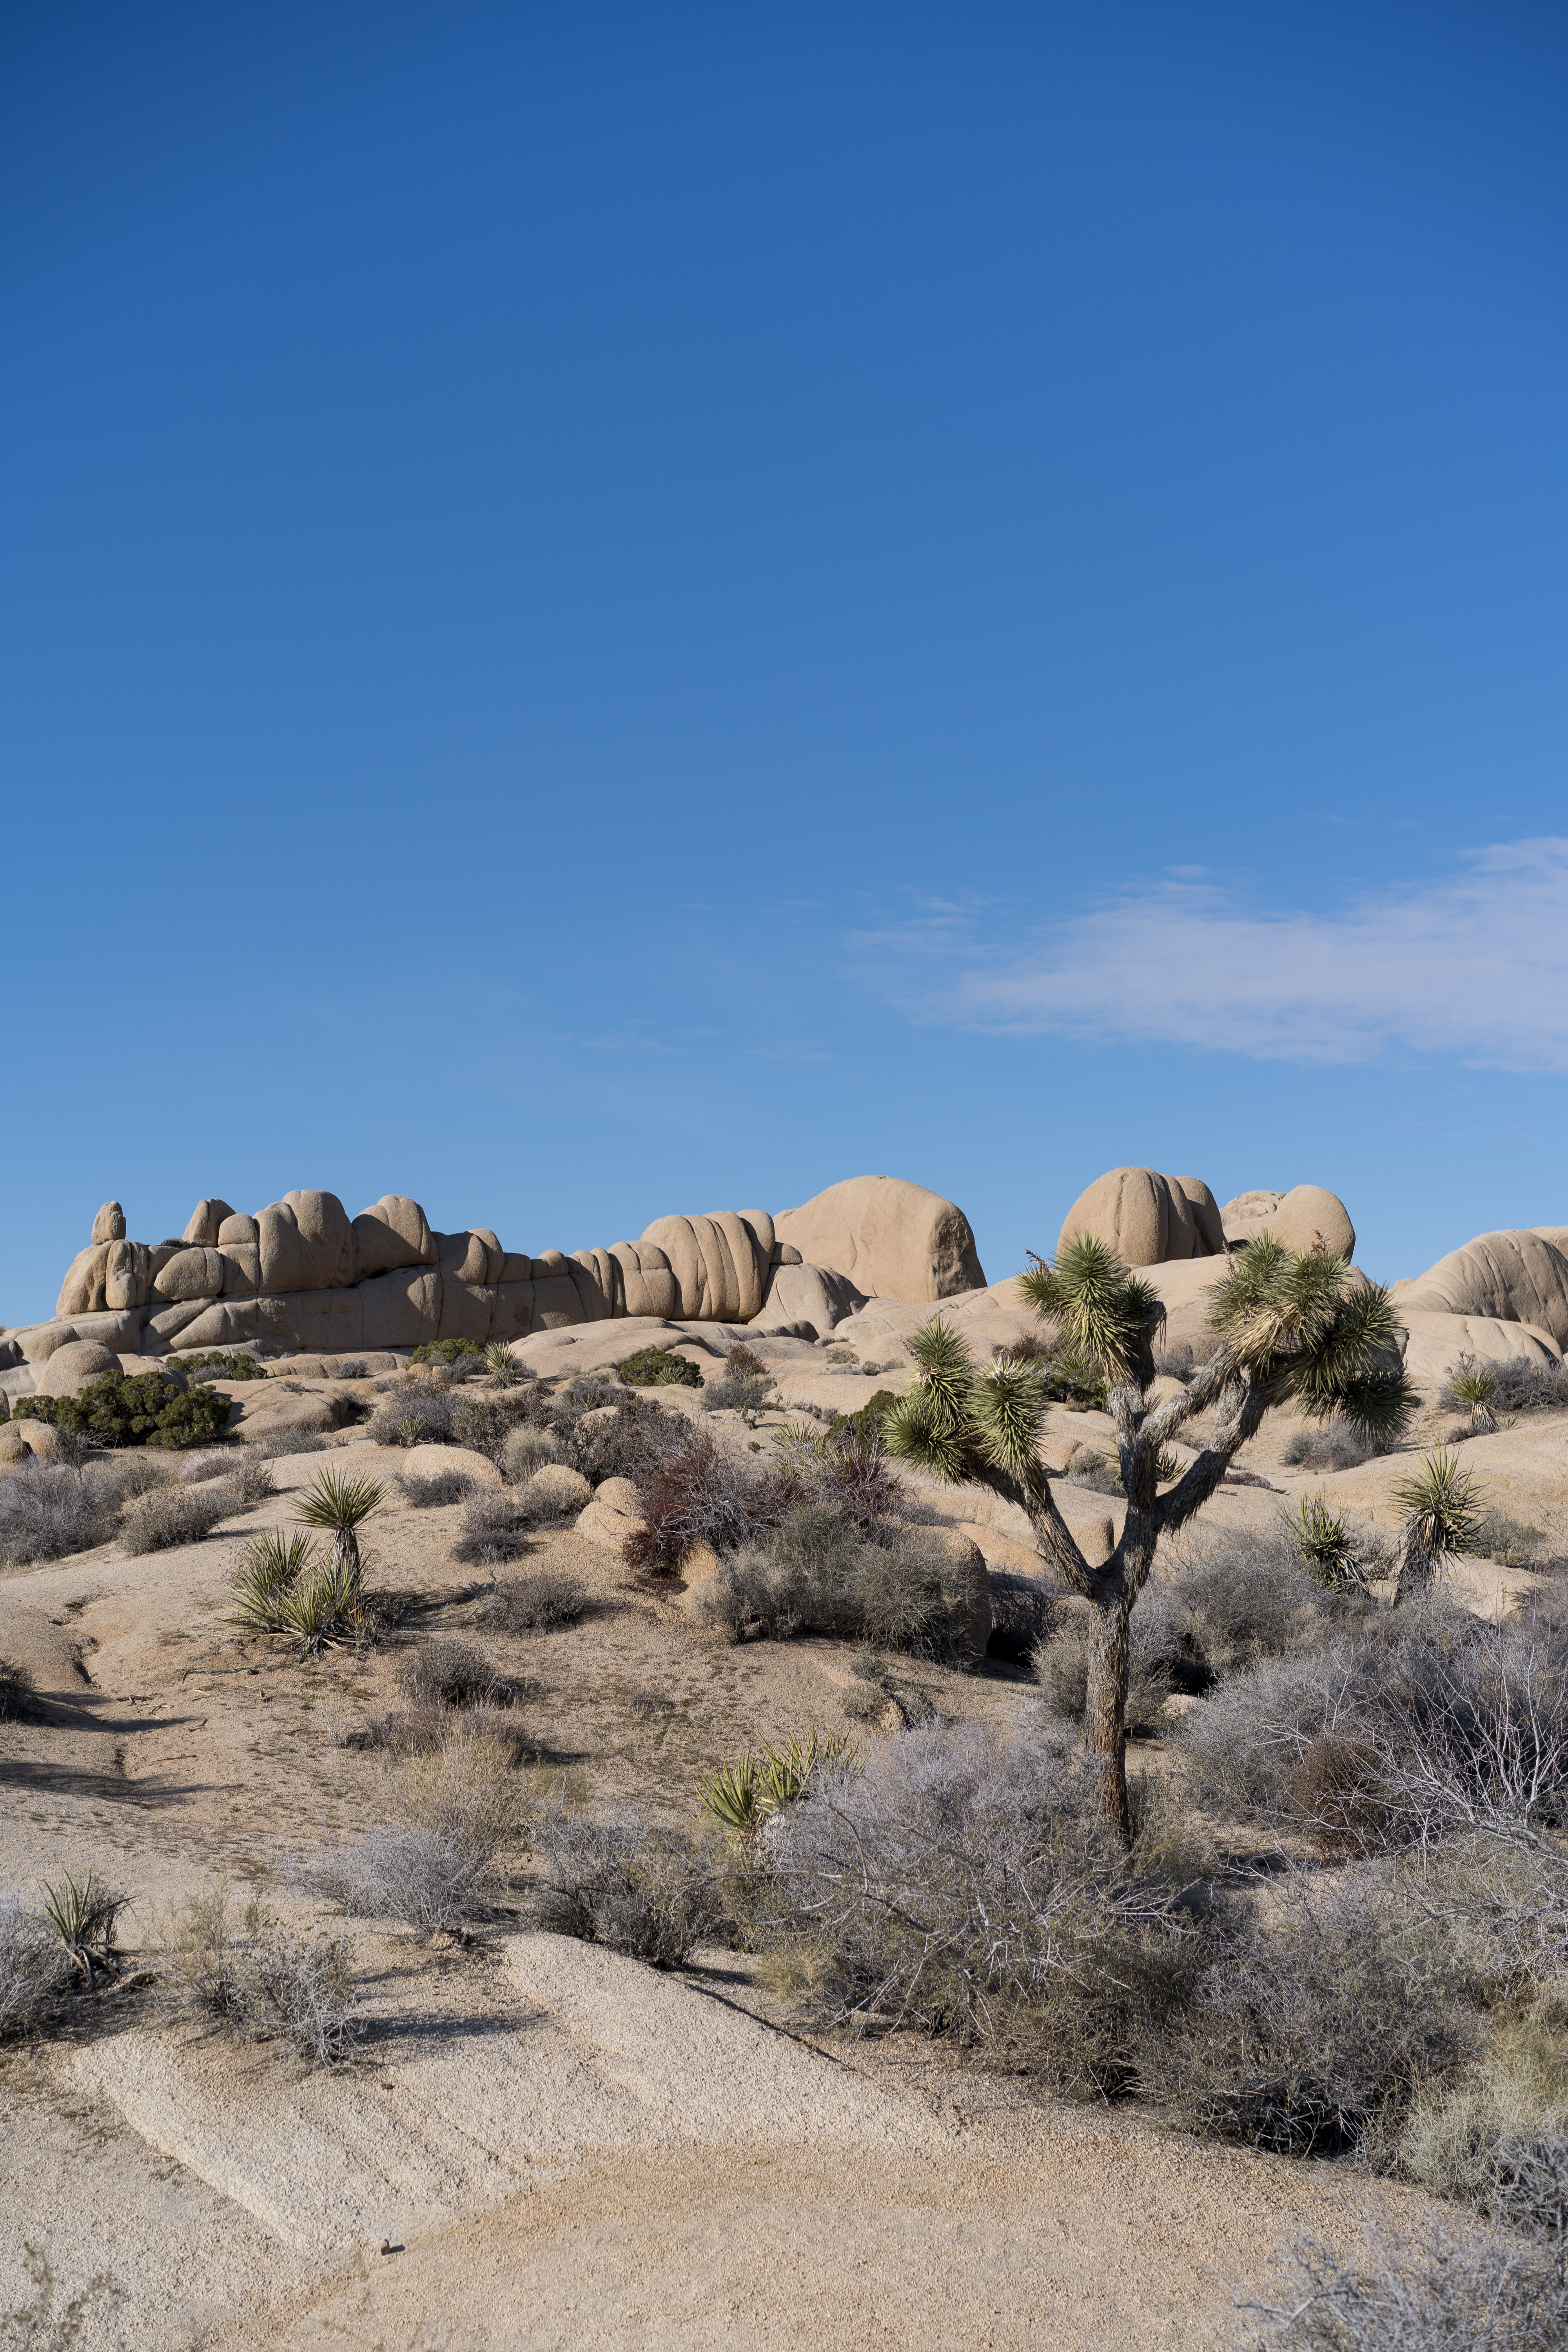
\includegraphics[width=\textwidth]{../Resource/image.png}
        \caption{Original}
        \label{fig:image-linear-original}
    \end{subfigure}
    \hfill
    \begin{subfigure}[b]{0.32\textwidth}
        \centering
        \includegraphics[width=\textwidth]{../Result/Linear/linear-bsc-output.png}
        \caption{Without correction}
        \label{fig:image-linear-no-correction}
    \end{subfigure}
    \hfill
    \begin{subfigure}[b]{0.32\textwidth}
        \centering
        \includegraphics[width=\textwidth]{../Result/Linear/linear-bsc-output-syndrome-corrected.png}
        \caption{Corrected}
        \label{fig:image-linear-syndrome-corrected}
    \end{subfigure}
       \caption{Image encoded with (7, 4) linear Hamming code (entire)}
       \label{fig:image-linear}
\end{figure}


\begin{figure}[htb]
    \centering
    \begin{subfigure}[b]{0.32\textwidth}
        \centering
        \includegraphics[width=\textwidth]{../Resource/cropped-image.png}
        \caption{Original}
        \label{fig:cropped-image-linear-original}
    \end{subfigure}
    \hfill
    \begin{subfigure}[b]{0.32\textwidth}
        \centering
        \includegraphics[width=\textwidth]{../Result/Linear/cropped-linear-bsc-output.png}
        \caption{Without correction}
        \label{fig:cropped-image-linear-no-correction}
    \end{subfigure}
    \hfill
    \begin{subfigure}[b]{0.32\textwidth}
        \centering
        \includegraphics[width=\textwidth]{../Result/Linear/cropped-linear-bsc-output-syndrome-corrected.png}
        \caption{Corrected}
        \label{fig:cropped-image-linear-syndrome-corrected}
    \end{subfigure}
       \caption{Image encoded with (7, 4) linear Hamming code (details)}
       \label{fig:cropped-image-linear}
\end{figure}


\begin{figure}[htb]
    \centering
    % \begin{subfigure}[b]{\textwidth}
    %     \centering
    %     \includegraphics[width=\textwidth]{../Result/Linear/wav-time-domain-TX.png}
    %     \caption{Original}
    %     \label{fig:t-audio-linear-original}
    % \end{subfigure}
    % \hfill
    \begin{subfigure}[b]{\textwidth}
        \centering
        \includegraphics[width=\textwidth]{../Result/Linear/linear-bsc-wav-time-domain-RX.png}
        \caption{Without correction}
        \label{fig:t-audio-linear-no-correction}
    \end{subfigure}
    % \hfill
    \begin{subfigure}[b]{\textwidth}
        \centering
        \includegraphics[width=\textwidth]{../Result/Linear/linear-bsc-wav-time-domain-RX-syndrome-corrected.png}
        \caption{Corrected}
        \label{fig:t-audio-linear-syndrome-corrected}
    \end{subfigure}
       \caption{Audio encoded with (7, 4) linear Hamming code}
       \label{fig:t-audio-linear}
\end{figure}



\section{$(n,k)$ Systematic Cyclic Code}
The $(n,k)$ Systematic Cyclic Code is a powerful and widely used error correction code (ECC) in the field of digital communications and information theory. The notation $(n,k)$ denotes that each block of the code consists of '$n$' bits, where '$k$' bits are the actual information or data, and the remaining '$n-k$' bits are the parity or check bits used for error detection and correction.

The term "systematic" implies that the data bits remain in their original form in the encoded output, while the parity bits are appended to form the full code word. This is in contrast to non-systematic coding schemes, where the data and parity bits are intermixed.

"Cyclic" codes, meanwhile, have a key property where a cyclic shift of a code word results in another valid code word. This cyclic nature leads to efficient implementation, especially in hardware, as simple shift registers can be used.

When the linear error-correcting codes is able to correct only single-bit errors in codewords, they are also called "Hamming" code. They accomplish this by introducing additional parity bits that allow the identification of single-bit errors.

In the context of $(n,k)$ Systematic Cyclic Codes, the codes are designed such that any $t$-bit error can be detected and corrected, making them a reliable choice for environments where such errors are common and the integrity of information is paramount.


\subsection{Adjustable $(n,k)$ for correcting $t$ errors}
\label{sec:adjustable-nk}
Allowing for a customizable n and k required many complex steps but we will work from the base all the way up to the overall algorithm.
\subsubsection{Polynomial Representation}
The first step is to represent polynomials in an efficient manner. While the rest of the code uses a numpy array to represent everything, this section exclusively represents polynomials using integers, with each bit representing the coefficients. For example, the number 11 in binary is 0b1011. This means that the code will interpret 11 as the polynomial $x^3+x+1$.
\subsubsection{Polynomial Division}
Next we need to be able to divide polynomials. This was done with an algorithm similar to how you would divide by hand:
\begin{enumerate}
    \item Initialize the remainder to the dividend
    \item Left shift divisor so that top bits align with remainder
    \item Subtract the result of step 2 from the remainder.
    \item Set the bit in the quotient according to the number of bits shifted
    \item Repeat 2-4 until the remainder is less than the divisor.
\end{enumerate}
\subsubsection{Finding a Generator Polynomial}
The search for a generator polynomial relies on two mathematical facts. Firstly, for any $(n, k)$ cyclic code, the generator polynomial $g(X)$ fits the equation $X^n+1 = g(X)*h(X)$. This means that the generator polynomial must evenly divide $X^n+1$.  Additionally, the generator polynomial must have order $n-k$. Using these two facts as constraints, we can brute force search through possible generators until  a viable candidate is found.
\subsubsection{Building the Generator Matrix}
Normally, a generator matrix for cyclic codes can be easily built using cyclic shifts. However, building it in a systematic form requires extra care. Any block code can be converted to systematic form using row operations. Below is an example of the generation of a $(7,4)$ code.

\begin{flushleft}
Initial:
\[
\begin{bmatrix}
1 & 0 & 1 & 1 & 0 & 0 & 0 \\
\end{bmatrix}
\]

Right shift:
\[
\begin{bmatrix}
1 & 0 & 1 & 1 & 0 & 0 & 0 \\
0 & 1 & 0 & 1 & 1 & 0 & 0 \\
\end{bmatrix}
\]

Correct systematic:
\[
\begin{bmatrix}
1 & 0 & 1 & 1 & 0 & 0 & 0 \\
1 & 1 & 1 & 0 & 1 & 0 & 0 \\
\end{bmatrix}
\]

Right shift:
\[
\begin{bmatrix}
1 & 0 & 1 & 1 & 0 & 0 & 0 \\
1 & 1 & 1 & 0 & 1 & 0 & 0 \\
0 & 1 & 1 & 1 & 0 & 1 & 0 \\
\end{bmatrix}
\]

Correct systematic:
\[
\begin{bmatrix}
1 & 0 & 1 & 1 & 0 & 0 & 0 \\
1 & 1 & 1 & 0 & 1 & 0 & 0 \\
1 & 1 & 0 & 0 & 0 & 1 & 0 \\
\end{bmatrix}
\]

Right shift:
\[
\begin{bmatrix}
1 & 0 & 1 & 1 & 0 & 0 & 0 \\
1 & 1 & 1 & 0 & 1 & 0 & 0 \\
1 & 1 & 0 & 0 & 0 & 1 & 0 \\
0 & 1 & 1 & 0 & 0 & 0 & 1 \\
\end{bmatrix}
\]

Done
\end{flushleft}

\subsubsection{Checking the Correctable Errors}
The number of correctable errors for a given code is based on the minimum distance between the codewords. The minimum distance of a code is equal to the minimum weight of all the codewords.
Finding the minimum wait codeword can be difficult since there are $2^k$ codewords. However, since this is a systematic code, every codeword will at least have a weight equal to the information encoded in it. This means we can guide our search by iterating through minimum weight information words. It will also stop the search preemptively if the weight of the information words becomes larger than an already determined minimum. With a minimum distance of $d$, the number correctable errors is $(d-1)//2$ 
\subsubsection{Overall Algorithm}
\begin{enumerate}
    \item Find a suitable generator polynomial given $n$ and $k$
    \item Build the generator matrix
    \item Check how many errors the code can correct
    \item If this does not meet the target correctable errors, repeat.
\end{enumerate}
This algorithm can also be modified to search for all possible generators and find the best one.

\subsection{Encoder}
The encoding process in a $(n,k)$ Systematic Cyclic Code involves the multiplication of a $k$-bit message vector with a generator matrix. The generator matrix for a $(n,k)$ Cyclic Code, in its systematic form, is given as:
% \begin{equation*}
%     G = 
%     \begin{bmatrix}
%         1 & 1 & 0 & 0 & 1 & 0 & 0 & 0 & 0 & 0 & 0 & 0 & 0 & 0 & 0 \\
%         0 & 1 & 1 & 0 & 0 & 1 & 0 & 0 & 0 & 0 & 0 & 0 & 0 & 0 & 0 \\
%         0 & 0 & 1 & 1 & 0 & 0 & 1 & 0 & 0 & 0 & 0 & 0 & 0 & 0 & 0 \\
%         1 & 1 & 0 & 1 & 0 & 0 & 0 & 1 & 0 & 0 & 0 & 0 & 0 & 0 & 0 \\
%         1 & 0 & 1 & 0 & 0 & 0 & 0 & 0 & 1 & 0 & 0 & 0 & 0 & 0 & 0 \\
%         0 & 1 & 0 & 1 & 0 & 0 & 0 & 0 & 0 & 1 & 0 & 0 & 0 & 0 & 0 \\
%         1 & 1 & 1 & 0 & 0 & 0 & 0 & 0 & 0 & 0 & 1 & 0 & 0 & 0 & 0 \\
%         0 & 1 & 1 & 1 & 0 & 0 & 0 & 0 & 0 & 0 & 0 & 1 & 0 & 0 & 0 \\
%         1 & 1 & 1 & 1 & 0 & 0 & 0 & 0 & 0 & 0 & 0 & 0 & 1 & 0 & 0 \\
%         1 & 0 & 1 & 1 & 0 & 0 & 0 & 0 & 0 & 0 & 0 & 0 & 0 & 1 & 0 \\
%         1 & 0 & 0 & 1 & 0 & 0 & 0 & 0 & 0 & 0 & 0 & 0 & 0 & 0 & 1
%     \end{bmatrix}
% \end{equation*}
\begin{equation*}
    G = \begin{bmatrix}
        P & I_{k}
    \end{bmatrix}
\end{equation*}
where $I_k$ represents a $k$ by $k$ identity matrix, and $P$ represents a $k$ by $(n-k)$ matrix for parity-check bits. 

Following is an example of the generator matrix for a $(15,11)$ Cyclic Hamming Code ($t=1$), which is generated with procedures in Section~\ref{sec:adjustable-nk}:
\begin{equation*}
    G = 
    \begin{bmatrix}
        1 & 1 & 0 & 0 & 1 & 0 & \cdots & 0 & 0 \\
        0 & 1 & 1 & 0 & 0 & 1 & \cdots & 0 & 0 \\
        \vdots & \vdots & \vdots & \vdots & \vdots & \vdots & \ddots & \vdots & \vdots \\
        1 & 0 & 1 & 1 & 0 & 0 & \cdots & 1 & 0 \\
        1 & 0 & 0 & 1 & 0 & 0 & \cdots & 0 & 1 \\
    \end{bmatrix} .
\end{equation*}

If we denote the message vector as 
\begin{equation*}
    u =
        \begin{bmatrix}
        u_1 & u_2 & \dots & u_k 
        \end{bmatrix},
\end{equation*}
then the encoded codeword $v$ is computed by:
\begin{equation*}
    v = u \cdot G .
\end{equation*}

This multiplication produces a $n$-bit codeword, which is then ready for transmission.


\subsection{Syndrome Decoder}
When there are only 1-bit errors in the received codewords, the error bit can be corrected by using the syndrome lookup table with the following general strategy. 

First, the parity-check matrix $H$ will be created from the generator matrix $G$ by transposing the $k$ by $(n-k)$ parity-check bits and filling it with an $(n-k)$ by $(n-k)$ identity matrix:
\begin{equation*}
    H = \begin{bmatrix}
        I_{n-k} & P^T
    \end{bmatrix} .
\end{equation*}

The decoding process of the $(n, k)$ cyclic code for $t=1$ error involves utilizing a syndrome lookup table, which is generated from the matrix multiplication:
\begin{equation*}
\text{syndrome table} = e \cdot H^T = \begin{bmatrix}
0_{1\times n} \\
I_n
\end{bmatrix} \cdot H^T .
\end{equation*}
where the $n$ by $n$ identity matrix with an extra row of zeros on the top, $e$, represents all the possible error patterns which are correctable by a syndrome look-up table for this specific $(n, k)$ cyclic code with generator matrix $G$. Each row of $e$ represents an error pattern identified by the same row of syndrome table. 

Following is an example of the parity-check matrix $H$ and syndrome look-up table for a (15, 11) Cyclic Hamming Code ($t=1$):
\begin{equation*}
H = 
\begin{bmatrix}
1 & 0 & 0 & 0 & 1 & 0 & \dots & 1 & 1 \\
0 & 1 & 0 & 0 & 1 & 1 & \dots & 0 & 0 \\
0 & 0 & 1 & 0 & 0 & 1 & \dots & 1 & 0 \\
0 & 0 & 0 & 1 & 0 & 0 & \dots & 1 & 1 \\
\end{bmatrix} ,
\end{equation*}
\begin{equation}
\text{syndrome table} = 
\begin{bmatrix}
0 & 0 & 0 & 0 \\
1 & 0 & 0 & 0 \\
0 & 1 & 0 & 0 \\
\vdots & \vdots & \vdots & \vdots \\
1 & 0 & 1 & 1 \\
1 & 0 & 0 & 1 \\
\end{bmatrix} .
\end{equation}



When a codeword is received, the syndrome $s$ is computed from the received bits and is used to identify the error pattern:
\begin{equation*}
    s = r \cdot H^T ,
\end{equation*}
where the $r = [r_1\  r_2\  \dots\  r_n ]$ represents the received codeword. 

Each syndrome corresponds to a potential error pattern in the look-up table. The estimated transmitted codeword can be calculated by modulo 2 addiction of error pattern and received codeword:
\begin{equation*}
    \tilde{v} = r + e[i:] \mod 2 ,
\end{equation*}
where the $e[i:]$ represents the $i$-th row of error patterns $e$ when the calculated syndrome $s$ matches the $i$-th row of the syndrome table. 

Since the code we are working on is systematic code, messages can be directly extracted from the last $k$ bits of codewords. 


\subsubsection{Results: TXT, PNG, WAV}

\begin{table}[htb]
    \centering
    \caption{Text string encoded with (15, 11) cyclic code with 1 correctable error (syndrome decoder)}
    \label{tab:text-cyclic-15-11-syndrome}
    \renewcommand{\arraystretch}{1.5}
    \begin{tabulary}{\textwidth}{ |L|L|L| } 
    \hline
    \textbf{Original} & \textbf{Without correction} & \textbf{Corrected} \\
    \hline
    Hello World! EEC269A Error Correcting Code Demo & H\textcolor{red}{u,}lo World! EEC269A Error Correcti\textcolor{red}{f}g Code Demo & Hello World! EEC269A Error Correcting Code Demo \\
    \hline
    \end{tabulary}
\end{table}


\begin{figure}[htb]
    \centering
    \begin{subfigure}[b]{0.32\textwidth}
        \centering
        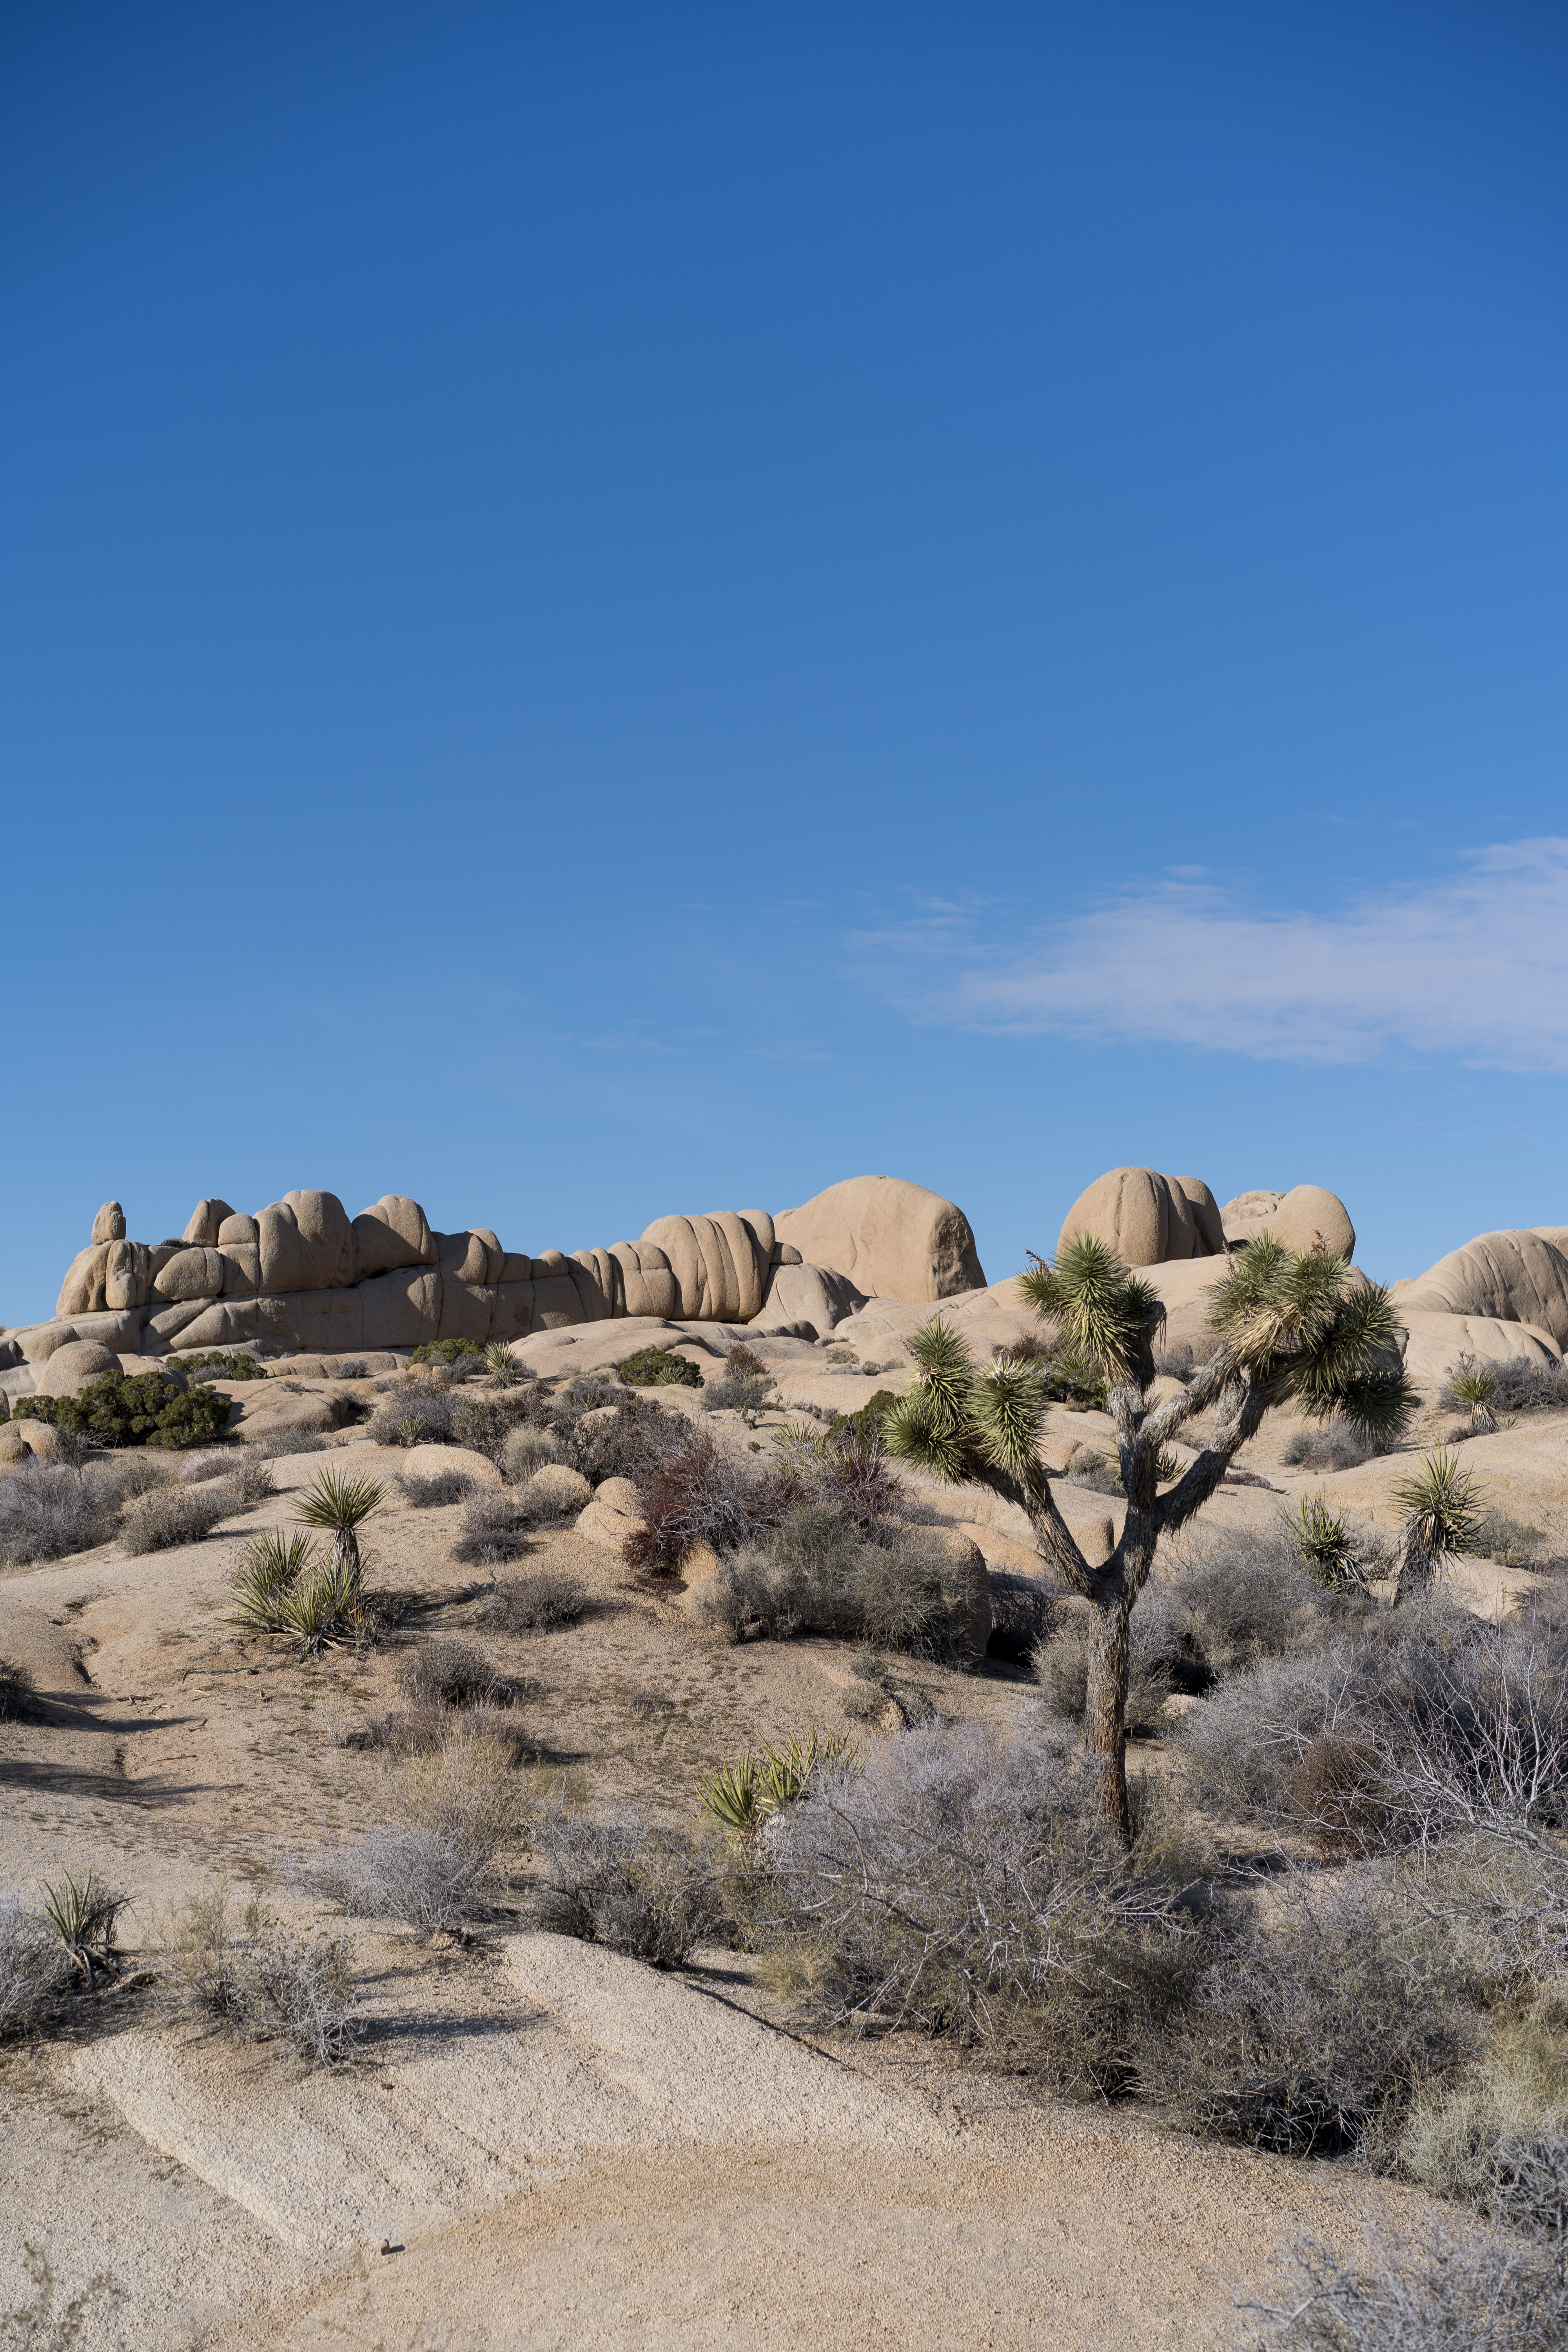
\includegraphics[width=\textwidth]{../Resource/image.png}
        \caption{Original}
        \label{fig:image-cyclic-15-11-original}
    \end{subfigure}
    \hfill
    \begin{subfigure}[b]{0.32\textwidth}
        \centering
        \includegraphics[width=\textwidth]{../Result/Cyclic/15-11/cyclic-bsc-output.png}
        \caption{Without correction}
        \label{fig:image-cyclic-15-11-no-correction}
    \end{subfigure}
    \hfill
    \begin{subfigure}[b]{0.32\textwidth}
        \centering
        \includegraphics[width=\textwidth]{../Result/Cyclic/15-11/cyclic-bsc-output-syndrome-corrected.png}
        \caption{Corrected}
        \label{fig:image-cyclic-15-11-syndrome-corrected}
    \end{subfigure}
       \caption{Image encoded with (15, 11) cyclic code with 1 correctable error (syndrome decoder) (entire)}
       \label{fig:image-cyclic-15-11-syndrome}
\end{figure}




\begin{figure}[htb]
    \centering
    \begin{subfigure}[b]{0.32\textwidth}
        \centering
        \includegraphics[width=\textwidth]{../Resource/cropped-image.png}
        \caption{Original}
        \label{fig:cropped-image-cyclic-15-11-original}
    \end{subfigure}
    \hfill
    \begin{subfigure}[b]{0.32\textwidth}
        \centering
        \includegraphics[width=\textwidth]{../Result/Cyclic/15-11/cropped-cyclic-bsc-output.png}
        \caption{Without correction}
        \label{fig:cropped-image-cyclic-15-11-no-correction}
    \end{subfigure}
    \hfill
    \begin{subfigure}[b]{0.32\textwidth}
        \centering
        \includegraphics[width=\textwidth]{../Result/Cyclic/15-11/cropped-cyclic-bsc-output-syndrome-corrected.png}
        \caption{Corrected}
        \label{fig:cropped-image-cyclic-15-11-syndrome-corrected}
    \end{subfigure}
       \caption{Image encoded with (15, 11) cyclic code with 1 correctable error (syndrome decoder) (details)}
       \label{fig:cropped-image-cyclic-15-11-syndrome}
\end{figure}




\begin{figure}[htb]
    \centering
    % \begin{subfigure}[b]{\textwidth}
    %     \centering
    %     \includegraphics[width=\textwidth]{../Result/Cyclic/15-11/wav-time-domain-TX.png}
    %     \caption{Original}
    %     \label{fig:t-audio-cyclic-15-11-original}
    % \end{subfigure}
    % \hfill
    \begin{subfigure}[b]{\textwidth}
        \centering
        \includegraphics[width=\textwidth]{../Result/Cyclic/15-11/cyclic-bsc-wav-time-domain-RX.png}
        \caption{Without correction}
        \label{fig:t-audio-cyclic-15-11-no-correction}
    \end{subfigure}
    % \hfill
    \begin{subfigure}[b]{\textwidth}
        \centering
        \includegraphics[width=\textwidth]{../Result/Cyclic/15-11/cyclic-bsc-wav-time-domain-RX-syndrome-corrected.png}
        \caption{Corrected}
        \label{fig:t-audio-cyclic-15-11-syndrome-corrected}
    \end{subfigure}
       \caption{Audio encoded with (15, 11) cyclic code with 1 correctable error (syndrome decoder)}
       \label{fig:t-audio-cyclic-15-11-syndrome}
\end{figure}









\subsection{Error Trapping Decoder}
When there are 1-bit errors or more than one bit errors in the received codewords, the error bits can be corrected by error trapping decoder with the following general strategy.

This decoder starts off the same as the syndrome LUT decoder. It uses the parity matrix to calculate the syndrome of the codeword. If the syndrome is zero, then the word has no errors and is passed to the output.

That is where the similarities end. To correct any errors, the decoder uses the syndrome itself as the error pattern. If the syndrome has weight less than or equal to the amount of errors the code can correct, then the syndrome can be added to the top portion of the codeword to remove any errors.

If the weight of the syndrome is too high, then the decoder performs a cyclic shift on the codeword and tries again. Eventually, the decoder will reach a correctable state. After fixing the error, the cyclic shifts are undone and it is passed to the output.

If the decoder shifts through the whole codeword without finding a correctable syndrome, the codeword is deemed uncorrectable. For our case, we decided to simply ignore the error and pass the erroneous codeword to the output.


Here is an example:

Let's say for a given $(15,7)$ code with $t=2$, the received codeword is:
\[
    [1\ 1\ 0\ 0\ 0\ 0\ 1\ 0\ 0\ 0\ 0\ 1\ 1\ 0\ 1]
\]

This has a resulting syndrome of:
\[
    [1\ 1\ 1\ 0\ 1\ 0\ 0\ 0]
\]
which has a weight greater than 2, meaning that the error cannot be corrected. 

However, after a cyclic shift, the codeword and syndrome become:
\begin{equation*}
    \begin{split}
        &[1\ 0\ 0\ 0\ 0\ 1\ 0\ 0\ 0\ 0\ 1\ 1\ 0\ 1\ 1] \\
        &\implies [0\ 0\ 0\ 0\ 0\ 0\ 0\ 1]
    \end{split}
\end{equation*}

This now a correctable pattern and the decoder repair the codeword as follows:

Original: 
\[
    [1\ 1\ 0\ 0\ 0\ 0\ 1\ 0\ 0\ 0\ 0\ 1\ 1\ 0\ 1]
\]

Shift 1: 
\[
    [1\ 0\ 0\ 0\ 0\ 1\ 0\ 0\ 0\ 0\ 1\ 1\ 0\ 1\ 1]
\]

Correct:
\[
    [1\ 0\ 0\ 0\ 0\ 1\ 0\ 1\ 0\ 0\ 1\ 1\ 0\ 1\ 1]
\]

Shift -1:
\[
    [1\ 1\ 0\ 0\ 0\ 0\ 1\ 0\ 1\ 0\ 0\ 1\ 1\ 0\ 1]
\]


\subsubsection{Results: TXT, PNG, WAV}

\begin{table}[htb]
    \centering
    \caption{Text string encoded with (15, 5) cyclic code with 3 correctable error (error trapping decoder)}
    \label{tab:text-cyclic-15-5-trapping}
    \renewcommand{\arraystretch}{1.5}
    \begin{tabulary}{\textwidth}{ |L|L|L| } 
    \hline
    \textbf{Original} & \textbf{Without correction} & \textbf{Corrected} \\
    \hline
    Hello World! EEC269A Error Correcting Code Demo & Hello World! EEC26\textcolor{red}{\textsuperscript{A}} Error Co\textcolor{red}{`}recting C\textcolor{red}{"}de Dem\textcolor{red}{k} & Hello World!
    EEC269A Error Correcting Code Demo \\
    \hline
\end{tabulary}
\end{table}


% Results : CRC (15 ,5) - error trapping method for .png file
\begin{figure}[htb]
    \centering
    \begin{subfigure}[b]{0.32\textwidth}
        \centering
        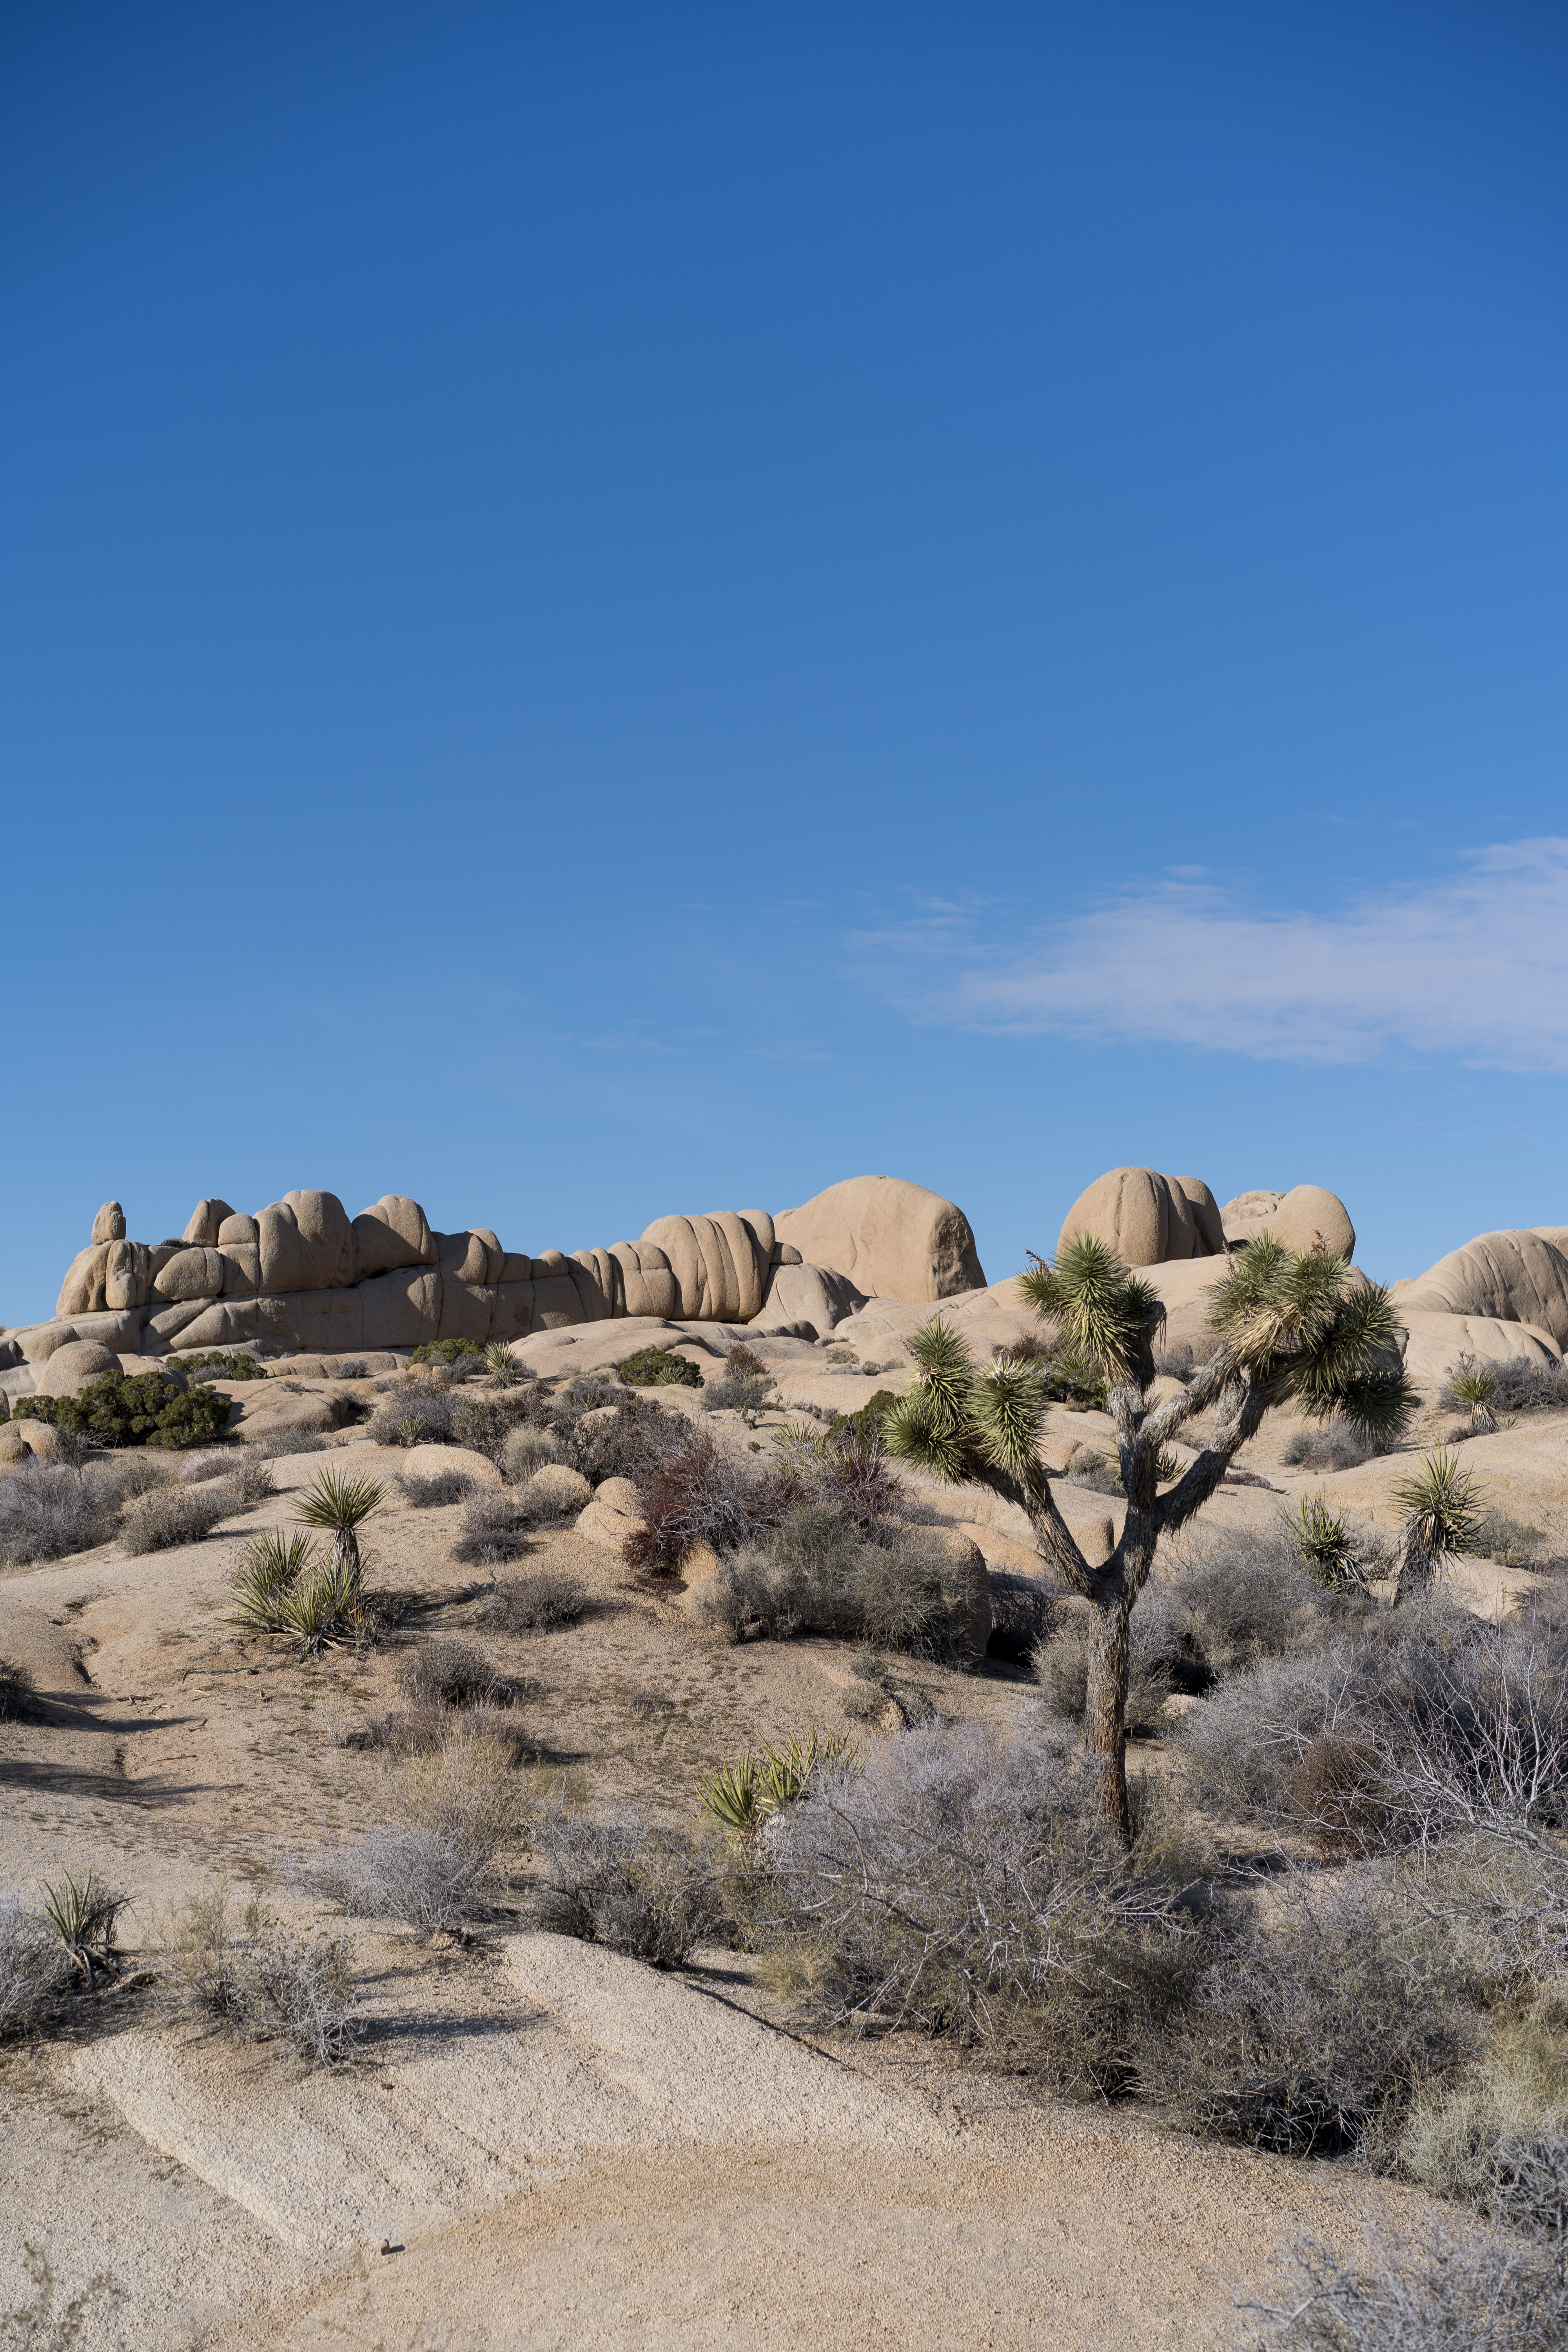
\includegraphics[width=\textwidth]{../Resource/image.png}
        \caption{Original}
        \label{fig:image-cyclic-15-5-original}
    \end{subfigure}
    \hfill
    \begin{subfigure}[b]{0.32\textwidth}
        \centering
        \includegraphics[width=\textwidth]{../Result/Cyclic/15-5/cyclic-bsc-output.png}
        \caption{Without correction}
        \label{fig:image-cyclic-15-5-no-correction}
    \end{subfigure}
    \hfill
    \begin{subfigure}[b]{0.32\textwidth}
        \centering
        \includegraphics[width=\textwidth]{../Result/Cyclic/15-5/cyclic-bsc-output-trapping-corrected.png}
        \caption{Corrected}
        \label{fig:image-cyclic-15-5-trapping-corrected}
    \end{subfigure}
       \caption{Image encoded with (15, 5) cyclic code with 3 correctable error (error trapping decoder) (details)}
       \label{fig:image-cyclic-15-5-trapping}
\end{figure}


\begin{figure}[htb]
    \centering
    \begin{subfigure}[b]{0.32\textwidth}
        \centering
        \includegraphics[width=\textwidth]{../Resource/cropped-image.png}
        \caption{Original}
        \label{fig:cropped-image-cyclic-15-5-original}
    \end{subfigure}
    \hfill
    \begin{subfigure}[b]{0.32\textwidth}
        \centering
        \includegraphics[width=\textwidth]{../Result/Cyclic/15-5/cropped-cyclic-bsc-output.png}
        \caption{Without correction}
        \label{fig:cropped-image-cyclic-15-5-no-correction}
    \end{subfigure}
    \hfill
    \begin{subfigure}[b]{0.32\textwidth}
        \centering
        \includegraphics[width=\textwidth]{../Result/Cyclic/15-5/cropped-cyclic-bsc-output-trapping-corrected.png}
        \caption{Corrected}
        \label{fig:cropped-image-cyclic-15-5-trapping-corrected}
    \end{subfigure}
       \caption{Image encoded with (15, 5) cyclic code with 3 correctable error (error trapping decoder) (details)}
       \label{fig:cropped-image-cyclic-15-5-trapping}
\end{figure}


% Results : CRC (15 ,5) - error trapping method for .wav file
\begin{figure}[htb]
    \centering
    % \begin{subfigure}[b]{\textwidth}
    %     \centering
    %     \includegraphics[width=\textwidth]{../Result/Cyclic/15-5/wav-time-domain-TX.png}
    %     \caption{Original}
    %     \label{fig:t-audio-cyclic-15-5-original}
    % \end{subfigure}
    % \hfill
    \begin{subfigure}[b]{\textwidth}
        \centering
        \includegraphics[width=\textwidth]{../Result/Cyclic/15-5/cyclic-bsc-wav-time-domain-RX.png}
        \caption{Without correction}
        \label{fig:t-audio-cyclic-15-5-no-correction}
    \end{subfigure}
    % \hfill
    \begin{subfigure}[b]{\textwidth}
        \centering
        \includegraphics[width=\textwidth]{../Result/Cyclic/15-5/cyclic-bsc-wav-time-domain-RX-trapping-corrected.png}
        \caption{Corrected}
        \label{fig:t-audio-cyclic-15-5-trapping-corrected}
    \end{subfigure}
       \caption{Audio encoded with (15, 5) cyclic code with 3 correctable error (error trapping decoder)}
       \label{fig:t-audio-cyclic-15-5-trapping}
\end{figure}

 
% \newpage
% \section{Appendix: Python source code}
% \subsection{Source}
% \label{appendix:source}
% \lstinputlisting[language=Python]{../Code/source.py}

% \subsection{Channel}
% \label{appendix:channel}
% \lstinputlisting[language=Python]{../Code/channel.py}

% \subsection{Destination}
% \label{appendix:destination}
% \lstinputlisting[language=Python]{../Code/destination.py}

% \subsection{Utilities}
% \label{appendix:utils}
% \lstinputlisting[language=Python]{../Code/Utils/polyTools.py}
% \lstinputlisting[language=Python]{../Code/Utils/plot_wav.py}
% \lstinputlisting[language=Python]{../Code/Utils/stat_analysis.py}

% \subsection{Linear code}
% \label{appendix:linear-code}
% \lstinputlisting[language=Python]{../Code/linear-code.py}

% \subsection{Cyclic code}
% \label{appendix:cyclic-code}
% \lstinputlisting[language=Python]{../Code/cyclic-code.py}

\section{Statistics Analysis}

In this section, we discuss the statistical results of all the 3 coding and decoding approaches that we had in this project. The results for (7, 4) Hamming code are brought in Table \ref{tab:stat-linear}. Accordingly, the bit error rate for all file types (including text, image, and audio file) is almost the same which is equal to the error probability of the binary symmetric channel (BSC with $p = 0.01$). The linear hamming code is capable of correcting up to 1 error per codeword. Consequently, the bit error rate is decreased to a certain amount after correction. However, some errors remain uncorrected. 

We show the results for (15, 5) cyclic code with error trapping decoder and (15, 11) cyclic code with syndrome decoder in Table \ref{tab:stat-trapping-(15,5)} and Table \ref{tab:stat-syndrome-(15,11)}, respectively. These 2 approaches compete with each other in a trade-off between accuracy and transmission rate concepts. Hence, we decide to use the coding technique according to the problem requirements and there is no perfect coding that can satisfy the mentioned metrics at the maximum possible value simultaneously. The (15,11) Cyclic code can correct up to 1 error per codeword, while the (15,5) Cyclic code corrects up to 3 errors. However, the total codewords generated by the (15, 11) CRC is 35, and this value is equal to 75 codewords (more than twice) for the (15, 5) CRC. Consequently, we need more time or bandwidth to transfer the same file with the second technique. It is worth mentioning that the final bit error rates (after correction) of these 2 models are equal to 0.0000 for text files, which indicates that the (15, 11) outperforms the (15, 5) due to its lower bandwidth/time consumption. But for larger data types, like audio or image files, the after-correction error rate of  (15,11) is less than (15,5), which promises a more reliable communication.

\begin{table}[htb]
    \centering
    \caption{Statistic results of (7,4) linear Hamming code}
    \label{tab:stat-linear}
    \renewcommand{\arraystretch}{1.5}
    \begin{tabulary}{\textwidth}{|L|L|L|L|}
    \hline
    \textbf{File Type} & \textbf{Metric} & \textbf{Before Correction} & \textbf{After Correction} \\
    \hline
    \multirow{8}{*}{TXT} & Total codewords & 94 & - \\
     & Correct codewords & 88 & - \\
     & Codeword error rate & 0.063830 & - \\
     & \qquad 1 error codewords & 6 & - \\
     & \qquad Uncorrectable codewords & 0 & - \\
     & Number of correct bits & 372 & 376 \\
     & Number of incorrect bits & 4 & 0 \\
     & Bit error rate & 0.010638 & 0.000000 \\
    \hline
    \multirow{8}{*}{PNG} & Total codewords & 6558720 & - \\
     & Correct codewords & 6113686 & - \\
     & Codeword error rate & 0.067854 & - \\
     & \qquad 1 error codewords & 431981 & - \\
     & \qquad Uncorrectable codewords & 13053 & - \\
     & Number of correct bits & 25973102 & 26212419 \\
     & Number of incorrect bits & 261778 & 22461 \\
     & Bit error rate & 0.009978 & 0.000856 \\
    \hline
    \multirow{8}{*}{WAV} & Total codewords & 2145896 & - \\
     & Correct codewords & 2000385 & - \\
     & Codeword error rate & 0.067809 & - \\
     & \qquad 1 error codewords & 141137 & - \\
     & \qquad Uncorrectable codewords & 4374 & - \\
     & Number of correct bits & 8497569 & 8576040 \\
     & Number of incorrect bits & 86015 & 7544 \\
     & Bit error rate & 0.010021 & 0.000879 \\
    \hline
    \end{tabulary}
\end{table}


\begin{table}[htb]
    \centering
    \caption{Statistic results of (15, 11) cyclic code with 1 correctable error (syndrome decoder)}
    \label{tab:stat-syndrome-(15,11)}
    \renewcommand{\arraystretch}{1.5}
    \begin{tabulary}{\textwidth}{|L|L|L|L|}
    \hline
    \textbf{File Type} & \textbf{Metric} & \textbf{Before Correction} & \textbf{After Correction} \\
    \hline
    \multirow{8}{*}{TXT} & Total codewords & 35 & - \\
     & Correct codewords & 29 & - \\
     & Codeword error rate & 0.171429 & - \\
     & \qquad 1 error codewords & 6 & - \\
     & \qquad Uncorrectable codewords & 0 & - \\
     & Number of correct bits & 372 & 376 \\
     & Number of incorrect bits & 4 & 0 \\
     & Bit error rate & 0.010638 & 0.000000 \\
    \hline
    \multirow{8}{*}{PNG} & Total codewords & 2384990 & - \\
     & Correct codewords & 2051296 & - \\
     & Codeword error rate & 0.139914 & - \\
     & \qquad 1 error codewords & 310904 & - \\
     & \qquad Uncorrectable codewords & 22790 & - \\
     & Number of correct bits & 25972541 & 26184088 \\
     & Number of incorrect bits & 262339 & 50792 \\
     & Bit error rate & 0.010000 & 0.001936 \\
    \hline
    \multirow{8}{*}{WAV} & Total codewords & 780326 & - \\
     & Correct codewords & 671482 & - \\
     & Codeword error rate & 0.139485 & - \\
     & \qquad 1 error codewords & 101430 & - \\
     & \qquad Uncorrectable codewords & 7414 & - \\
     & Number of correct bits & 8497796 & 8567137 \\
     & Number of incorrect bits & 85788 & 16447 \\
     & Bit error rate & 0.009994 & 0.001916 \\
    \hline
    \end{tabulary}
\end{table}



\begin{table}[htb]
    \centering
    \caption{Statistic results of (15, 5) cyclic code with 3 correctable error (error trapping decoder)}
    \label{tab:stat-trapping-(15,5)}
    \renewcommand{\arraystretch}{1.5}
    \begin{tabulary}{\textwidth}{|L|L|L|L|}
    \hline
    \textbf{File Type} & \textbf{Metric} & \textbf{Before Correction} & \textbf{After Correction} \\
    \hline
    \multirow{10}{*}{TXT} & Total codewords & 76 & - \\
     & Correct codewords & 64 & - \\
     & Codeword error rate & 0.157895 & - \\
     & \qquad 1 error codewords & 11 & - \\
     & \qquad 2 error codewords & 1 & - \\
     & \qquad 3 error codewords & 0 & - \\
     & \qquad Uncorrectable codewords & 0 & - \\
     & Number of correct bits & 372 & 376 \\
     & Number of incorrect bits & 4 & 0 \\
     & Bit error rate & 0.010638 & 0.000000 \\
    \hline
    \multirow{10}{*}{PNG} & Total codewords & 5246976 & - \\
     & Correct codewords & 4514112 & - \\
     & Codeword error rate & 0.139674 & - \\
     & \qquad 1 error codewords & 682449 & - \\
     & \qquad 2 error codewords & 48298 & - \\
     & \qquad 3 error codewords & 2051 & - \\
     & \qquad Uncorrectable codewords & 66 & - \\
     & Number of correct bits & 25972642 & 26234721 \\
     & Number of incorrect bits & 262238 & 159 \\
     & Bit error rate & 0.009996 & 0.000006 \\
    \hline
    \multirow{10}{*}{WAV} & Total codewords & 1716717 & - \\
     & Correct codewords & 1476183 & - \\
     & Codeword error rate & 0.140113 & - \\
     & \qquad 1 error codewords & 223879 & - \\
     & \qquad 2 error codewords & 15896 & - \\
     & \qquad 3 error codewords & 731 & - \\
     & \qquad Uncorrectable codewords & 28 & - \\
     & Number of correct bits & 8497463 & 8583525 \\
     & Number of incorrect bits & 86121 & 59 \\
     & Bit error rate & 0.010033 & 0.000007 \\
    \hline
    \end{tabulary}
\end{table}





\section{Other Challenges}
\subsection{Why PNG and WAV}
The primary difference between file formats such as PNG and JPEG, or WAV and MP3, is the way the data is compressed. More specifically, the difference is in whether the compression is lossless or lossy.

**PNG vs JPEG:**

PNG uses a lossless compression algorithm, meaning that when the image data is compressed and then decompressed, there is no loss of information. The image remains exactly the same as the original.

On the other hand, JPEG uses a lossy compression algorithm. This means that some data is lost when the image is compressed and then decompressed. JPEG's algorithm reduces file size by discarding some of the less important data or information that's less perceivable to the human eye. This results in smaller file sizes which is beneficial for web usage or storing many photos where high fidelity isn't the priority. However, the image quality decreases with the level of compression, potentially leading to noticeable artifacts or blurring.

**WAV vs MP3:**

Similarly, WAV (Waveform Audio File Format) and MP3 (MPEG-1 Audio Layer III) are both audio file formats that differ in their compression methods.

WAV files are a raw audio format created by Microsoft and IBM. They are lossless, uncompressed, and retain full quality of the audio data. This results in high-quality audio but also significantly larger file sizes. It's commonly used in professional settings where high audio quality is a must, like music production or broadcasting.

MP3, however, uses a form of lossy data compression to encode data using inexact approximations, significantly reducing the file size. It was designed to greatly reduce the amount of data required to represent audio, yet still sound like a faithful reproduction of the original uncompressed audio to most listeners. This has made it a common format for consumer audio streaming and storage, but the lossy nature means that some audio fidelity is sacrificed for smaller file size.

In summary, the choice between these formats depends on your needs. If retaining the original quality of the image or sound is of utmost importance, then lossless formats like PNG and WAV are the way to go. However, if you need to save storage space or bandwidth and can afford some loss in quality, then lossy formats like JPEG and MP3 would be more suitable.



\subsection{Why only extract DATA chunk}
When we talk about chunks in the context of PNG and WAV files, we're referring to sections of data within these files that have different purposes. In both file types, each chunk begins with a header that identifies its type and carries other relevant information such as the chunk's size. The way these chunks are handled contributes significantly to how these file types work. But what happens if these chunks get messed up? Let's take a closer look.

**PNG:**

In a PNG file, the chunks store different types of data such as the image's metadata, palette data, and actual image data (in the IDAT chunk), among other things. 

If a chunk other than the IDAT chunk is messed up or corrupted, the PNG viewer or editor will still attempt to display the image data. However, depending on the severity and location of the corruption, different issues may arise. 

For example, if the IHDR chunk (header chunk containing crucial details like width, height, bit depth, etc.) is corrupted, the image may not display correctly or at all, because these fundamental details are required to interpret the image data correctly. A corrupted PLTE chunk (palette data) might result in wrong colors being displayed. 

If ancillary chunks like tEXt (textual information), pHYs (physical pixel dimensions), or tIME (last modification time) are corrupted, it's less severe since these chunks do not directly affect the display of the image, but it may cause incorrect metadata to be displayed or used.

**WAV:**

In a WAV file, data is also organized into chunks. The two primary chunks are the 'fmt ' chunk, containing format information like sample rate, bit depth, and number of channels, and the 'data' chunk, which contains the actual audio data.

Corruption or misinterpretation of the 'fmt ' chunk can result in the audio file being unplayable because the player wouldn't know how to correctly interpret the raw audio data. The audio could also be played back at the wrong speed, or with incorrect bit depth or number of channels, causing significant distortions or alterations to the sound.

Other optional chunks in a WAV file, such as 'LIST' (metadata), 'fact' (additional format information), or 'cue ' (cue points), might not prevent the audio from being played if they get messed up, but they could lead to loss of additional information or features associated with the audio file.

In both cases, it's essential to note that how severely the corruption of a chunk impacts the file can also depend on the software used to view or play the file, as different software may have different ways of handling such errors.


\subsection{Speed up program}
Loops in programming languages like Python can be slow, especially when iterating through large matrices. There are several ways we can speed up a for loop when performing matrix operations:

\begin{enumerate}
\item \textbf{Use NumPy library:} NumPy is a library in Python specifically designed to handle numerical computations much faster than Python's built-in methods, mainly when dealing with matrices or arrays. NumPy performs operations in compiled C code under the hood, making it much more efficient. Suppose you have a matrix A and you want to add a vector v to each row. In a for loop, you might write:
\begin{verbatim}
for i in range(A.shape[0]):
    A[i, :] += v
\end{verbatim}
But with NumPy, you can write:
\begin{verbatim}
A += v
\end{verbatim}
This will perform the addition in a vectorized manner, which is much faster than using a for loop.

\item \textbf{Use Broadcasting:} Broadcasting is a powerful mechanism that allows NumPy to work with arrays of different shapes when performing arithmetic operations. You can often use broadcasting to eliminate the need for loops entirely.

\item \textbf{Use Vectorized Operations:} Instead of using loops, you can often rephrase your problem in a way that allows you to use vectorized operations. These are operations that are performed on whole arrays at once, which can be much faster than looping through individual elements.

\item \textbf{Parallelize your code:} If your loop iterations are independent (i.e., the result of one iteration doesn't depend on the result of any other), you might be able to speed up your code significantly by running multiple iterations in parallel. Libraries like \textit{joblib} and \textit{multiprocessing} can help with this in Python.

\end{enumerate}






\end{document}